\documentclass[a4paper,12pt]{article}
% Define paper size, seperate titlepage, 12 pt. font, document class
%--------------------------------------------------------------------------------------------------
% Begin Preamble
%--------------------------------------------------------------------------------------------------
\usepackage{amsmath}
\usepackage{amssymb}
\usepackage{here}
\usepackage{graphicx}
\usepackage{epstopdf}
\usepackage{framed}
\usepackage{stmaryrd}
\usepackage{amsthm}
\usepackage{multicol}
\usepackage{manfnt}
\usepackage{fancybox}
\usepackage{pdflscape}
\usepackage{epsfig}
\usepackage{multirow}
\usepackage{color}
\usepackage{booktabs}
\usepackage{natbib}
\usepackage{lettrine}
\usepackage{appendix}
\usepackage{ifthen}
\usepackage[affil-it]{authblk}
\usepackage[utf8]{inputenc}
\usepackage[T1]{fontenc}
\usepackage{kpfonts}
\usepackage[doublespacing]{setspace}
\usepackage{csquotes}
\usepackage{subcaption}
%\usepackage{booktabs}
%\usepackage{threeparttable}
% Load Standard Packages
\usepackage{tabularx}
\newcolumntype{Y}{>{\centering\arraybackslash}X}
%Graphs and Tables to the end of the paper
\usepackage{endfloat}
\usepackage{array}
\usepackage[section]{placeins}
\usepackage[table,xcdraw]{xcolor}
\usepackage{longtable}
\usepackage{rotating}
\definecolor{maroon}{rgb}{0.62, 0.15, 0.20}
\definecolor{timberwolf}{rgb}{0.86, 0.84, 0.82}
\definecolor{navy}{rgb}{0.05, 0.27, 0.44}

%--------------------------------------------------------------------------------------------------
\usepackage{setspace}
	\onehalfspacing
% Set spacing to 1.5
%\numberwithin{figure}{section}
%\numberwithin{table}{section}
%  Number within Sections

\definecolor{deepred}{rgb}{0.803922,0,0}
%--------------------------------------------------------------------------------------------------
\usepackage{fancyhdr}
	\pagestyle{fancy}
	\headheight 35pt
	\fancyhf{}
	\rhead{}
	\chead{}
	\lhead{}
	\lhead{}
	\rfoot{\thepage}
	\cfoot{}
	\lfoot{}
	\renewcommand{\headrulewidth}{0.0pt}
	\renewcommand{\footrulewidth}{0.0pt}
% Define header and footnote styles
%--------------------------------------------------------------------------------------------------
%\usepackage[small,bf]{caption}
%\setlength{\captionmargin}{20pt}
% Makes the captions of figures/tables look nicely
%--------------------------------------------------------------------------------------------------
\usepackage[flushleft]{threeparttable}
\usepackage{ifxetex}
%\usepackage[dvipsnames]{xcolor}
\ifxetex{%
  \usepackage{fontspec}
  \setmainfont{Linux Libertine O} % or any font on your system
  \newfontfamily\quotefont[Ligatures=TeX]{Linux Libertine O} % or any font on your system
\else
  \usepackage[utf8]{inputenc}
  \usepackage[T1]{fontenc}
  \usepackage{kpfonts} % or any other font package (or none)
  \newcommand*\quotefont{\fontfamily{fxl}} % selects Libertine for quote font
\fi
\usepackage{tikz}
\usepackage{framed}
% Make commands for the quotes
\newcommand*{\openquote}{\tikz[remember picture,overlay,xshift=-15pt,yshift=-10pt]
     \node (OQ) {\quotefont\fontsize{60}{60}\selectfont``};\kern0pt}
\newcommand*{\closequote}{\tikz[remember picture,overlay,xshift=15pt,yshift=10pt]
     \node (CQ) {\quotefont\fontsize{60}{60}\selectfont''};}
% select a colour for the shading

% wrap everything in its own environment
\newenvironment{shadequote}%
{\begin{snugshade}\begin{quote}\openquote}
{\hfill\closequote\end{quote}\end{snugshade}}
%--------------------------------------------------------------------------------------------------
\usepackage[margin=2.3cm,includeheadfoot=false,twoside=false,bindingoffset=0.0cm,showframe=false]{geometry}
%\fancyhfoffset[E,O]{0pt}
% Add nicer enumbering of formulars
%--------------------------------------------------------------------------------------------------
\newcommand{\ws}{$^{\,\star}$}
\newcommand{\ms}{$^{\,\star \star}$}
\newcommand{\hs}{$^{\,\star \star \star}$}
\newcommand{\sym}[1]{\rlap{#1}}
% End Preamble
%--------------------------------------------------------------------------------------------------
\title{The Political Economy of European Asylum Policies}
\date{December 2017}
\author[,1]{Martina Burmann\thanks{burmann@ifo.de}}
\author[,1]{Marcus Drometer\thanks{drometer@ifo.de}}
\author[,2]{Romuald M\'eango\thanks{meango@mea.mpisoc.mpg.de}}
\affil[1]{ifo Institute for Economic Research, Munich}
\affil[2]{Munich Center for the Economics of Aging (MEA)}
\renewcommand\Authands{ and }
%--------------------------------------------------------------------------------------------------
\begin{document}
%--------------------------------------------------------------------------------------------------
      \maketitle
%--------------------------------------------------------------------------------------------------

\begin{center}

\end{center}
\begin{abstract}
\singlespacing
\noindent 
Despite the recognition that asylum policies are partly determined by political economy factors in the destination country, there is little empirical evidence on the precise linkages between those political factors and asylum policies. We shed light on this issue by examining the impact of elections and parties on first-time asylum applications.  Our evidence is based on a large bilateral panel data set comprising 12 European destination countries and their 51 most relevant origin countries during the time period 2002 to 2014. Our findings suggest that  the number of asylum applicants under left- and right-wing parties converges before elections and differs thereafter. This result is robust to several different specifications and suggest that both left- and right-wing cabinets choose moderate policies before the election and less moderate policies after the election.

% MARTINA: maybe also add something about the decision analysis in the abstract %

\bigskip

\textbf{Keywords}: Electoral cycles, migration policies.

\textbf{JEL}: H11, D72, F22

\bigskip
\end{abstract}
%\addtolength{\baselineskip}{.25\baselineskip}
\setcounter{page}{0} \renewcommand{\thepage}{}
\pagebreak\pagenumbering{arabic}\pagebreak

%%--------------------------------------------------------------------------------------------------
\section{Introduction}\label{Introduction}
Since March 2016, the European Union has signed an agreement with Turkey to close off the migration route across the Aegean, one of the most popular routes for asylum-seekers from Asia. This has been done despite protests from many human rights groups that think such an agreement violates the international Convention on Refugees. In a tribune entitled ``Keep them away'', \textit{\cite{Economist2017}} describes policies intended by many EU countries as policies ``where asylum-seekers would need to apply from abroad rather than coming to Europe.'' This tension between the provision of asylum for rightfully entitled individuals and groups, and the pursuit of other political and economic goals has been acknowledged by the economic literature that compares the provision of asylum as a public good, where costs are privately assumed by the host countries \citep{moraga2014}. With this background in mind, \cite{dustmann2016} note that ``the  different  exposures  to  refugee  inflows and  the  lack  of  any  effective  European-level  mechanism  to  `spread  the  burden'  of  hosting  refugee  populations,  led  many  countries  to  implement  procedures  aimed  at  reducing  inflows  into  their  territories.''

[Hatton Economic Policy article]

Despite the recognition that asylum policies are partly determined by political economy factors in the destination country, there is little empirical evidence on the precise linkages between these factors. We shed light on this issue by examining the impact of elections on asylum applications and recognition rates based on a large bilateral panel data set for 12 European destination countries and 51 origin countries during the time period 2002 to 2014. Our findings suggest that asylum policies are affected by the electoral cycle and the identity of incumbent parties. More precisely, we establish two main results: (i) before an election, asylum policies are very similar across left-wing and right-wing cabinets; (ii)  in the quarters following an election, asylum policies diverge substantially, with a significantly lower inflow of refugees under a right-wing cabinet. This pattern suggests that both left- and right-wing cabinets choose moderate policies before the election to cater to the interests of the median voter and less moderate ones after the election implementing their preferred policies. 

With respect to the recognition rate, we also find that policies remain similar before the election, but differ thereafter. However, the recognition rate is lower under left-wing cabinets and higher under right-wing cabinets. Our interpretation is that changes in the number of applicants mechanically translate into changes in the recognition rate. If a right-wing government reduces the number of applicants by restricting access, the selection of asylum seeker that enter the country changes. This generates a pool of applicants that is more entitled to asylum and thus mechanically increase the recognition rate under a right-wing cabinet. This explanation is in line with our finding that the higher recognition rate under right-cabinets is not only driven by an increase of temporary protection but also by an increase in the number of applicant that obtain refugee status. 

We measure asylum policies in terms of policy outcomes, i.e., the number of applicants and the recognition rate. Both a country's asylum laws as well as their implementation by the ruling government determine these outcomes. While the existing literature focuses on legal determinants, we are the first to systematically asses how elections and changes in the government affect asylum policies. We find that both changes in asylum laws (as measured by Hatton's (2009) 
% MARTINA: Is that the correct citation for the index? we have it until 2014 so it is unlikely that it is from 2009, right? %
asylum policy index) as well as changes in the actual implementation by the ruling government matter. Detailed analysis suggest that our main results are driven by adjustments of access policies. Access policies, such as border controls, allow to regulate the flow of applicants, they can be changed rather quickly and are under the direct administration of the government. A current example is the close off of the migration route across the Aegean, one of the most popular routes for asylum-seekers from Asia, by the European Union in March 2016. This agreement between Turkey and the European Union drastically affected access for refugees without changing any national laws regarding asylum.\footnote{Another way to influence asylum policy outcomes is the level of enforcement of existing asylum laws. For example, ...} 

Even though asylum policy is less a matter of individual countries as during the 1980s and 1990s, the EU's attempt to build a Common European Asylum System (CEAS) is far from being completed (see \citet{hatton2015EU}). The individual EU member countries are left with substantial discretion regarding processing policies, e.g. safe third country provisions or deportations, and regarding the welfare benefits asylum seekers obtain which have a direct impact on the number of applicants a country receives.\footnote{For a detailed discussion of policy measures that deter asylum seekers and their effectiveness see \citet{thielemann2006}.} Additionally, access policies effectively still depend to a substantial extent on how national government interpret the Dublin Accord - during the period considered in our analysis and even more during the recent European refugee crisis.

 [and voucher schemes]

There are only very few country-specific studies that deal with impact of governments on immigration. \citet{gudbrandsen2010} analyzes partisan impact in the case of Norway refugee immigration to Norway and finds that refugee inflows are significantly LOWER? under conservative governments. Several studies evaluate how asylum policy changes affect asylum flows. For example, \citet{holzer2000} investigate whether the restrictive policies towards asylum seekers in Switzerland introduced around 1990 were successful in deterring migrants. Moreover, our paper is linked to the literature on the determinants of refugee inflows.\footnote{Among others see, e.g., \citep{neumayer2005, moore2007, hatton2009, hatton2016}} In line with existing findings, we confirm the importance of certain push factors in the origin country (e.g., political terror and civil war) as well as certain pull factors in the destination country (e.g., its labor market situation). Finally, our analysis relates to the literature on political budget cycles following \citet{nor75} which argues that incumbent politicians have strong incentives to distort public policies in order to increase approval rates whenever elections are pending. Finally,
%MARTINA: fianlly kommt schon im Satz davor, vielleicht To that extend ...%
 our analysis can be regarded as a test of whether parties converge to the interests of the median voter (\citet{downs1957}) or implement the policies they favor on ideological grounds (\citet{hibbs1977} and \citet{alesina1987}).

%\footnote{For a detailed survey on partisan politics see \citet{potrafke2017}.}.\footnote{In a related study, \citet{krause2017} find evidence that the number of deportations of foreigners that are obliged to leave the country depends on the ideology of the government.} 

The remainder of the paper proceeds as follows: Section \ref{sec:data} introduces the data used for our analysis. Section \ref{sec:econometric} presents the econometric framework, and section \ref{sec:results} discusses our main results. Then, section \ref{sec:robustness} provides several robustness checks. Finally, section \ref{sec:conclusion} concludes.

\section{Data} \label{sec:data}

We use quarterly data on the number of first-time asylum applications and decisions on asylum applications which is available from Eurostat. For our empirical analysis we select destination countries based on both data availability and size of the countries in the time period 2002 to 2014. More precisely, our main specification comprises all countries which have data on origin-specific first-time asylum applications in at least 44 out of the 52 quarters under study and which report in total more than 30000 first-time asylum applications between 2002 and 2014.\footnote{If countries have missing information in 2008 or 2009 we impute this data from data on the origin-specific total applications in the respective quarters. This information is only available from 2008 onwards and, therefore, it is not possible to impute missing information for the years before 2008. For the exact calculation see the data section in the online appendix.} Unfortunately, information regarding decisons on asylum applications is not available for the same countries in all relevant years. Thus our decision sample comprises fewer countries as evident from Table \ref{ftapp_and_dec_by_destination} which lists all countries used in our analysis.

\begin{table}[!ht]\centering \footnotesize
\caption{Total number of first-time asylum applications and decisions 2002 - 2014}
\begin{tabularx}{\textwidth}{lYY}
\hline\hline
Destination country & Number of first-time applications & Number of asylum decisions \\
\hline
Germany        	& 704,450 	& 587,635 \\
[0,5em]
France			& 629,272 	& 595,820 \\
[0,5em]
United Kingdom 	& 470,960 	& 461,295 \\
[0,5em]
Sweden 			& 445,525 	& 366,315 \\
[0,5em]
Belgium        	& 184,200 	& 		 \\
[0,5em]
Netherlands		& 167,055 	& 		 \\
[0,5em]
Norway        	& 113,545 	& 		 \\
[0,5em]
Poland			& 89,680 	& 49,305	 \\
[0,5em]
Denmark        	& 59,440 	& 35,485 \\
[0,5em]
Ireland			& 47,070 	& 37,330 \\	
[0,5em]
Czech Republic	& 35,370		& 29,820 \\			
\hline\hline
\multicolumn{3}{p{0.98\textwidth}}{\scriptsize Note: The number of first-time applications represent the sum of  first-time applications in all available quarters from Quarter 1 2002 to Quarter 4 2014. For France the number of first-time applications in 2008 and for  Spain the number of first-time applications in 2008 and 2009 are imputed from the number of origin-specific applications in these years. For Belgium no data is available in 2004 and for Norway no data is available in 2002 and in Quarter 2, 3 and 4 of 2007. The number of asylum decisions represent the sum of all positive and all rejected decisions in all available quarters from Quarter 1 2002 to Quarter 4 2014. For Ireland and Denmark no data is available in 2002. For France no data is available in 2007 and for Ireland, Spain and the United Kingdom no data is available in Quarter 4 of 2007.}
\end{tabularx}
\label{ftapp_and_dec_by_destination}
\end{table}

We further select the top 51 origin countries which together account for more than 90\% of all first-time applications in the 12 destination countries between 2002 and 2014. As evident from Table \ref{origin_countries} the top 10 origin countries already account for more than 45\% of the total first-time applications.\footnote{A full list of all 51 origin countries is provided in the online appendix.} Following \cite{hatton2016}, we drop country pairs with very few applications in order to avoid cases with zero applications in many quarters. Thus, we keep only country pairs with at least two first-time asylum applications per quarter on average, which leaves us with 480 out of 612 possible origin destination combinations. Similarly for the smaller sample of 9 destination countries that we use when analysing the decisions of asylum applications, we select the top 49 origin countries which together account for more than 90\% of all decisions taken in the 9 destination countries between 2002 and 2014. Moreover, we also drop country pairs with less than two decisions per quarter on average, which leaves us with 323 out of the 441 possible origin destination combinations in the decision analysis.


\begin{table}[!ht]\centering \footnotesize
\caption{Top 10 source countries}
\begin{tabularx}{\textwidth}{lYYYY}
\hline \hline
& \multicolumn{2}{c}{\textbf{First-time applications}} & \multicolumn{2}{c}{\textbf{Asylum decisions}}  \\
\cmidrule(lr){2-3} \cmidrule(lr){4-5}
Source country & Total & Share  & Total & Share \\
\hline 
\smallskip
Russia & 210,882 & 7.0\% & 126,005 & 5,7\% \\
\smallskip
Iraq & 207,447 & 6.9\%  & 173,295 & 7.8\% \\
\smallskip
Syria & 181,800 & 6.1\%  & 113,565 & 5.1\%  \\
\smallskip
Afghanistan & 157,124 & 5.2\% & 112,370 & 5.1\% \\
\smallskip
Somalia & 137,378 & 4.6\% & 84,015 & 3.8\%  \\
\smallskip
Iran & 100,691 & 3.4\% & 81,665 & 3.7\%  \\
\smallskip
Turkey  & 100,646 & 3.4\% & 107,240 & 4.8\% \\
\smallskip 
Eritrea & 100,259 & 3.3\% & 47,755 & 2.2\% \\
\smallskip
Serbia & 90,869 & 3.0\% & 83,485 & 3.8\% \\
\smallskip
Democratic Republic of Congo  & 82829 & 2.8\% &70360 & 3.2\% \\
\hline \hline
\multicolumn{5}{p{0.98\textwidth}}{\scriptsize Note: Column 1 represents the sum of all first-time applications in the 12 European destination countries by citizens of the respective origin country in the years 2002 to 2014. Column 2 represents the share of these first-time applications in all first-time applications in the 12 destination countries from 2002 to 2014. Column 3 shows the number of total asylum decisions for citizens from the respective origin country in the 9 destination countries for which decision data is available. Column 4 shows the respective share of these decisions in all asylum decisions taken in the 9 destination countries between 2002 and 2014. Note that the order of the top 10 origin countries for the decisions is slightly different than that of the applications, as the sample of destination countries differs. Moreover, Eritrea is not in the top 10 of the origin countries in terms of asylum decisions. Instead China is in the top 10 origin countries for asylum decision.}
\end{tabularx}
\label{origin_countries}
\end{table}

We combine the Eurostat dataset with the ParlGov dataset that comprises information on European national elections and party positions \citep{parlgov2016}. For our analysis, we both make use of the election date as well as changes in the position of the government on a left-right scale in the destination countries. Figure \ref{elections} illustrates the time-line of elections and cabinet changes as well as the before- and after-election periods as defined in our analysis (see below).\footnote{Note that only cabinet changes where the cabinet group switches between left and right are marked in the graph. There are many more small cabinet changes which do not cause a change in the cabinet position group.}


\begin{figure}	
\caption{Elections and cabinet changes}
\small
\centering
\renewcommand{\arraystretch}{0.5}
\scalebox{.7}{%
\begin{tabular}{l*{27}{c}}
	\parbox[0pt][2em]{0cm}{} & \multicolumn{4}{c}{\cellcolor{timberwolf} \normalsize 2002} & \multicolumn{4}{c}{\cellcolor{white} \normalsize 2003} & \multicolumn{4}{c}{\cellcolor{timberwolf} \normalsize 2004} & \multicolumn{4}{c}{ \cellcolor{white} \normalsize 2005} & \multicolumn{4}{c}{\cellcolor{timberwolf} \normalsize 2006} & \multicolumn{4}{c}{\cellcolor{white} \normalsize 2007} & \multicolumn{2}{c}{\cellcolor{timberwolf} \normalsize 2008}\\
	
		     & \cellcolor{timberwolf} 1 & \cellcolor{timberwolf} 2 & \cellcolor{timberwolf} 3 & \cellcolor{timberwolf} 4 & \cellcolor{white} 1 & \cellcolor{white} 2 & \cellcolor{white} 3 & \cellcolor{white} 4 & \cellcolor{timberwolf} 1 & \cellcolor{timberwolf} 2 & \cellcolor{timberwolf} 3 & \cellcolor{timberwolf} 4 & 1 & 2 & 3 & 4 & \cellcolor{timberwolf} 1 & \cellcolor{timberwolf} 2 & \cellcolor{timberwolf} 3 & \cellcolor{timberwolf} 4 & 1 & 2 & 3 & 4 & \cellcolor{timberwolf} 1 & \cellcolor{timberwolf} 2\\ \hline\hline
		     
	{\normalsize Belgium} \parbox[0pt][2em]{0cm}{}  & \cellcolor{maroon} - & \cellcolor{maroon} - & \cellcolor{maroon} - & \cellcolor{maroon} - & \cellcolor{maroon} - &  \cellcolor{maroon} \textbf{X} & \cellcolor{maroon} + & \cellcolor{maroon} + & \cellcolor{maroon} + & \cellcolor{maroon} + & \cellcolor{maroon} + & \cellcolor{maroon} + & \cellcolor{maroon} & \cellcolor{maroon} & \cellcolor{maroon} & \cellcolor{maroon}  - & \cellcolor{maroon} - & \cellcolor{maroon} - & \cellcolor{maroon} - & \cellcolor{maroon} - & \cellcolor{maroon} - & \cellcolor{maroon} \textbf{X} & \cellcolor{maroon} + & \cellcolor{maroon} + & \cellcolor{maroon} + & \cellcolor{maroon} +\\
	
	     & \cellcolor{timberwolf} & \cellcolor{timberwolf}& \cellcolor{timberwolf}& \cellcolor{timberwolf} & \cellcolor{white} & \cellcolor{white} & \cellcolor{white} & \cellcolor{white} & \cellcolor{timberwolf} & \cellcolor{timberwolf}& \cellcolor{timberwolf}& \cellcolor{timberwolf} & \cellcolor{white} & \cellcolor{white} & \cellcolor{white} & \cellcolor{white} & \cellcolor{timberwolf} & \cellcolor{timberwolf}& \cellcolor{timberwolf}& \cellcolor{timberwolf} & \cellcolor{white} & \cellcolor{white} & \cellcolor{white} & \cellcolor{white} & \cellcolor{timberwolf} & \cellcolor{timberwolf}\\
	     
	{\normalsize Czech Republic} \parbox[0pt][2em]{0cm}{} & \cellcolor{maroon} - & \cellcolor{maroon} \textbf{X} & \cellcolor{maroon} + & \cellcolor{maroon} + & \cellcolor{maroon} + & \cellcolor{maroon} + & \cellcolor{maroon} + & \cellcolor{maroon} + & \cellcolor{maroon} & \cellcolor{maroon} & \cellcolor{maroon} & \cellcolor{maroon} - & \cellcolor{maroon} - & \cellcolor{maroon} - & \cellcolor{maroon} - & \cellcolor{maroon} - & \cellcolor{maroon} - & \cellcolor{maroon} \textbf{X} & \cellcolor{maroon} + & \cellcolor{navy} + & \cellcolor{navy} + & \cellcolor{navy} + & \cellcolor{navy} + & \cellcolor{navy} + & \cellcolor{navy} & \cellcolor{navy}\\
	
		& \cellcolor{timberwolf} & \cellcolor{timberwolf}& \cellcolor{timberwolf}& \cellcolor{timberwolf} & \cellcolor{white} & \cellcolor{white} & \cellcolor{white} & \cellcolor{white} & \cellcolor{timberwolf} & \cellcolor{timberwolf}& \cellcolor{timberwolf}& \cellcolor{timberwolf} & \cellcolor{white} & \cellcolor{white} & \cellcolor{white} & \cellcolor{white} & \cellcolor{timberwolf} & \cellcolor{timberwolf}& \cellcolor{timberwolf}& \cellcolor{timberwolf} & \cellcolor{white} & \cellcolor{white} & \cellcolor{white} & \cellcolor{white} & \cellcolor{timberwolf} & \cellcolor{timberwolf}\\
		
	{\normalsize Denmark} \parbox[0pt][2em]{0cm}{} & \cellcolor{navy} + & \cellcolor{navy} + & \cellcolor{navy} + & \cellcolor{navy} + & \cellcolor{navy} + & \cellcolor{navy} + & \cellcolor{navy} & \cellcolor{navy} & \cellcolor{navy} & \cellcolor{navy} \textcolor{gray}{-} & \cellcolor{navy} \textcolor{gray}{-} & \cellcolor{navy} \textcolor{gray}{-} & \cellcolor{navy} \textcolor{gray}{\textbf{X}} & \cellcolor{navy} + & \cellcolor{navy} + & \cellcolor{navy} + & \cellcolor{navy} + & \cellcolor{navy} + & \cellcolor{navy} + & \cellcolor{navy} & \cellcolor{navy} & \cellcolor{navy} & \cellcolor{navy} \textcolor{gray}{-} & \cellcolor{navy} \textcolor{gray}{\textbf{X}} & \cellcolor{navy} + & \cellcolor{navy} +\\ 
	
	    & \cellcolor{timberwolf} & \cellcolor{timberwolf}& \cellcolor{timberwolf}& \cellcolor{timberwolf} & \cellcolor{white} & \cellcolor{white} & \cellcolor{white} & \cellcolor{white} & \cellcolor{timberwolf} & \cellcolor{timberwolf}& \cellcolor{timberwolf}& \cellcolor{timberwolf} & \cellcolor{white} & \cellcolor{white} & \cellcolor{white} & \cellcolor{white} & \cellcolor{timberwolf} & \cellcolor{timberwolf}& \cellcolor{timberwolf}& \cellcolor{timberwolf} & \cellcolor{white} & \cellcolor{white} & \cellcolor{white} & \cellcolor{white} & \cellcolor{timberwolf} & \cellcolor{timberwolf}\\
	    
	{\normalsize France} \parbox[0pt][2em]{0cm}{} & \cellcolor{maroon} - & \cellcolor{maroon} \textbf{X} & \cellcolor{navy} + & \cellcolor{navy} + & \cellcolor{navy} + & \cellcolor{navy} + & \cellcolor{navy} + & \cellcolor{navy} + & \cellcolor{navy} & \cellcolor{navy} & \cellcolor{navy} & \cellcolor{navy} & \cellcolor{navy} & \cellcolor{navy} & \cellcolor{navy} & \cellcolor{navy} - & \cellcolor{navy} - & \cellcolor{navy} - & \cellcolor{navy} - & \cellcolor{navy} - & \cellcolor{navy} - & \cellcolor{navy} \textbf{X} & \cellcolor{navy} + & \cellcolor{navy} + & \cellcolor{navy} + & \cellcolor{navy} +\\
	
		& \cellcolor{timberwolf} & \cellcolor{timberwolf}& \cellcolor{timberwolf}& \cellcolor{timberwolf} & \cellcolor{white} & \cellcolor{white} & \cellcolor{white} & \cellcolor{white} & \cellcolor{timberwolf} & \cellcolor{timberwolf}& \cellcolor{timberwolf}& \cellcolor{timberwolf} & \cellcolor{white} & \cellcolor{white} & \cellcolor{white} & \cellcolor{white} & \cellcolor{timberwolf} & \cellcolor{timberwolf}& \cellcolor{timberwolf}& \cellcolor{timberwolf} & \cellcolor{white} & \cellcolor{white} & \cellcolor{white} & \cellcolor{white} & \cellcolor{timberwolf} & \cellcolor{timberwolf}\\
		
	{\normalsize Germany} \parbox[0pt][2em]{0cm}{} & \cellcolor{maroon} - & \cellcolor{maroon} - & \cellcolor{maroon} \textbf{X} & \cellcolor{maroon} + & \cellcolor{maroon} + & \cellcolor{maroon} + & \cellcolor{maroon} + & \cellcolor{maroon} + & \cellcolor{maroon} + & \cellcolor{maroon}  & \cellcolor{maroon}  & \cellcolor{maroon}  & \cellcolor{maroon} \textcolor{gray}{-}  & \cellcolor{maroon} - & \cellcolor{maroon} \textcolor{gray}{\textbf{X}} & \cellcolor{maroon} + & \cellcolor{maroon} + & \cellcolor{maroon} + & \cellcolor{maroon} + & \cellcolor{maroon} + & \cellcolor{maroon} + & \cellcolor{maroon} & \cellcolor{maroon} & \cellcolor{maroon} & \cellcolor{maroon} - & \cellcolor{maroon} -\\ 
	
	     & \cellcolor{timberwolf} & \cellcolor{timberwolf}& \cellcolor{timberwolf}& \cellcolor{timberwolf} & \cellcolor{white} & \cellcolor{white} & \cellcolor{white} & \cellcolor{white} & \cellcolor{timberwolf} & \cellcolor{timberwolf}& \cellcolor{timberwolf}& \cellcolor{timberwolf} & \cellcolor{white} & \cellcolor{white} & \cellcolor{white} & \cellcolor{white} & \cellcolor{timberwolf} & \cellcolor{timberwolf}& \cellcolor{timberwolf}& \cellcolor{timberwolf} & \cellcolor{white} & \cellcolor{white} & \cellcolor{white} & \cellcolor{white} & \cellcolor{timberwolf} & \cellcolor{timberwolf}\\
	     
	{\normalsize Ireland} \parbox[0pt][2em]{0cm}{} & \cellcolor{navy} - & \cellcolor{navy} \textbf{X} & \cellcolor{navy} + & \cellcolor{navy} + & \cellcolor{navy} + & \cellcolor{navy} + & \cellcolor{navy} + & \cellcolor{navy} + & \cellcolor{navy}  & \cellcolor{navy} & \cellcolor{navy}  & \cellcolor{navy}  & \cellcolor{navy} & \cellcolor{navy} & \cellcolor{navy} & \cellcolor{navy} - & \cellcolor{navy} - & \cellcolor{navy} - & \cellcolor{navy} - & \cellcolor{navy} - & \cellcolor{navy} - & \cellcolor{navy} \textbf{X} & \cellcolor{maroon} + & \cellcolor{maroon} + & \cellcolor{maroon} + & \cellcolor{maroon} +\\
	
		& \cellcolor{timberwolf} & \cellcolor{timberwolf}& \cellcolor{timberwolf}& \cellcolor{timberwolf} & \cellcolor{white} & \cellcolor{white} & \cellcolor{white} & \cellcolor{white} & \cellcolor{timberwolf} & \cellcolor{timberwolf}& \cellcolor{timberwolf}& \cellcolor{timberwolf} & \cellcolor{white} & \cellcolor{white} & \cellcolor{white} & \cellcolor{white} & \cellcolor{timberwolf} & \cellcolor{timberwolf}& \cellcolor{timberwolf}& \cellcolor{timberwolf} & \cellcolor{white} & \cellcolor{white} & \cellcolor{white} & \cellcolor{white} & \cellcolor{timberwolf} & \cellcolor{timberwolf}\\
		
	{\normalsize Netherlands} \parbox[0pt][2em]{0cm}{} & \cellcolor{maroon}-  & \cellcolor{maroon} \textbf{X} & \cellcolor{navy} + & \cellcolor{navy} - & \cellcolor{navy} \textcolor{gray}{\textbf{X}}  & \cellcolor{navy} +  & \cellcolor{navy} + & \cellcolor{navy} + & \cellcolor{navy} + & \cellcolor{navy} + & \cellcolor{navy} + & \cellcolor{navy} & \cellcolor{navy} & \cellcolor{navy} & \cellcolor{navy} & \cellcolor{navy}  \textcolor{gray}{-} & \cellcolor{navy}  \textcolor{gray}{-} & \cellcolor{navy} -  & \cellcolor{navy} - & \cellcolor{navy} \textcolor{gray}{\textbf{X}} & \cellcolor{navy} +  & \cellcolor{maroon} + & \cellcolor{maroon} + & \cellcolor{maroon}  + & \cellcolor{maroon} +  & \cellcolor{maroon} + \\ 
	
    	& \cellcolor{timberwolf} & \cellcolor{timberwolf}& \cellcolor{timberwolf}& \cellcolor{timberwolf} & \cellcolor{white} & \cellcolor{white} & \cellcolor{white} & \cellcolor{white} & \cellcolor{timberwolf} & \cellcolor{timberwolf}& \cellcolor{timberwolf}& \cellcolor{timberwolf} & \cellcolor{white} & \cellcolor{white} & \cellcolor{white} & \cellcolor{white} & \cellcolor{timberwolf} & \cellcolor{timberwolf}& \cellcolor{timberwolf}& \cellcolor{timberwolf} & \cellcolor{white} & \cellcolor{white} & \cellcolor{white} & \cellcolor{white} & \cellcolor{timberwolf} & \cellcolor{timberwolf}\\
    	
	{\normalsize Norway} \parbox[0pt][2em]{0cm}{} & \cellcolor{navy} + & \cellcolor{navy} + & \cellcolor{navy} + & \cellcolor{navy} + & \cellcolor{navy} + & \cellcolor{navy} & \cellcolor{navy} & \cellcolor{navy} & \cellcolor{navy} - & \cellcolor{navy} - & \cellcolor{navy} - & \cellcolor{navy} - & \cellcolor{navy} - & \cellcolor{navy} - & \cellcolor{navy} \textbf{X} & \cellcolor{maroon}  + & \cellcolor{maroon} + & \cellcolor{maroon} + & \cellcolor{maroon} + & \cellcolor{maroon} + & \cellcolor{maroon} + & \cellcolor{maroon} & \cellcolor{maroon} & \cellcolor{maroon} & \cellcolor{maroon} - & \cellcolor{maroon} -\\
	
			& \cellcolor{timberwolf} & \cellcolor{timberwolf}& \cellcolor{timberwolf}& \cellcolor{timberwolf} & \cellcolor{white} & \cellcolor{white} & \cellcolor{white} & \cellcolor{white} & \cellcolor{timberwolf} & \cellcolor{timberwolf}& \cellcolor{timberwolf}& \cellcolor{timberwolf} & \cellcolor{white} & \cellcolor{white} & \cellcolor{white} & \cellcolor{white} & \cellcolor{timberwolf} & \cellcolor{timberwolf}& \cellcolor{timberwolf}& \cellcolor{timberwolf} & \cellcolor{white} & \cellcolor{white} & \cellcolor{white} & \cellcolor{white} & \cellcolor{timberwolf} & \cellcolor{timberwolf}\\
			
	{\normalsize Poland} \parbox[0pt][2em]{0cm}{} & \cellcolor{maroon} + & \cellcolor{maroon} + & \cellcolor{maroon} + & \cellcolor{maroon} + & \cellcolor{maroon} + & \cellcolor{maroon} & \cellcolor{maroon} & \cellcolor{maroon}  & \cellcolor{maroon} - & \cellcolor{maroon} - & \cellcolor{maroon} - & \cellcolor{maroon} - & \cellcolor{maroon} - & \cellcolor{maroon} - & \cellcolor{maroon} \textbf{X} & \cellcolor{navy} + & \cellcolor{navy} + & \cellcolor{navy} + & \cellcolor{navy} + & \cellcolor{navy} + & \cellcolor{navy} + & \cellcolor{navy} & \cellcolor{navy} - & \cellcolor{navy} \textcolor{gray}{\textbf{X}} & \cellcolor{navy} +  & \cellcolor{navy} +\\ 
	
	      & \cellcolor{timberwolf} & \cellcolor{timberwolf}& \cellcolor{timberwolf}& \cellcolor{timberwolf} & \cellcolor{white} & \cellcolor{white} & \cellcolor{white} & \cellcolor{white} & \cellcolor{timberwolf} & \cellcolor{timberwolf}& \cellcolor{timberwolf}& \cellcolor{timberwolf} & \cellcolor{white} & \cellcolor{white} & \cellcolor{white} & \cellcolor{white} & \cellcolor{timberwolf} & \cellcolor{timberwolf}& \cellcolor{timberwolf}& \cellcolor{timberwolf} & \cellcolor{white} & \cellcolor{white} & \cellcolor{white} & \cellcolor{white} & \cellcolor{timberwolf} & \cellcolor{timberwolf}\\
	      
	{\normalsize Spain} \parbox[0pt][2em]{0cm}{} & \cellcolor{navy}  & \cellcolor{navy}  & \cellcolor{navy} - & \cellcolor{navy} - & \cellcolor{navy} - & \cellcolor{navy} - & \cellcolor{navy} - & \cellcolor{navy} - & \cellcolor{navy} \textbf{X} & \cellcolor{maroon} + & \cellcolor{maroon} + & \cellcolor{maroon} + & \cellcolor{maroon} + & \cellcolor{maroon} + & \cellcolor{maroon} + & \cellcolor{maroon} & \cellcolor{maroon} & \cellcolor{maroon} & \cellcolor{maroon} - & \cellcolor{maroon} - & \cellcolor{maroon} - & \cellcolor{maroon} - & \cellcolor{maroon} - & \cellcolor{maroon} - & \cellcolor{maroon} \textbf{X} & \cellcolor{maroon} +\\
	
		& \cellcolor{timberwolf} & \cellcolor{timberwolf}& \cellcolor{timberwolf}& \cellcolor{timberwolf} & \cellcolor{white} & \cellcolor{white} & \cellcolor{white} & \cellcolor{white} & \cellcolor{timberwolf} & \cellcolor{timberwolf}& \cellcolor{timberwolf}& \cellcolor{timberwolf} & \cellcolor{white} & \cellcolor{white} & \cellcolor{white} & \cellcolor{white} & \cellcolor{timberwolf} & \cellcolor{timberwolf}& \cellcolor{timberwolf}& \cellcolor{timberwolf} & \cellcolor{white} & \cellcolor{white} & \cellcolor{white} & \cellcolor{white} & \cellcolor{timberwolf} & \cellcolor{timberwolf}\\
		
	{\normalsize Sweden} \parbox[0pt][2em]{0cm}{} & \cellcolor{maroon} - & \cellcolor{maroon} - & \cellcolor{maroon} \textbf{X} & \cellcolor{maroon} + & \cellcolor{maroon} + & \cellcolor{maroon} + & \cellcolor{maroon} + & \cellcolor{maroon} + & \cellcolor{maroon} + & \cellcolor{maroon} & \cellcolor{maroon} & \cellcolor{maroon} & \cellcolor{maroon} - & \cellcolor{maroon} - & \cellcolor{maroon} - & \cellcolor{maroon} - & \cellcolor{maroon} - & \cellcolor{maroon} - & \cellcolor{maroon} \textbf{X} & \cellcolor{navy} + & \cellcolor{navy} + & \cellcolor{navy} + & \cellcolor{navy} + & \cellcolor{navy} + & \cellcolor{navy} + & \cellcolor{navy}\\ 
	
	     & \cellcolor{timberwolf} & \cellcolor{timberwolf}& \cellcolor{timberwolf}& \cellcolor{timberwolf} & \cellcolor{white} & \cellcolor{white} & \cellcolor{white} & \cellcolor{white} & \cellcolor{timberwolf} & \cellcolor{timberwolf}& \cellcolor{timberwolf}& \cellcolor{timberwolf} & \cellcolor{white} & \cellcolor{white} & \cellcolor{white} & \cellcolor{white} & \cellcolor{timberwolf} & \cellcolor{timberwolf}& \cellcolor{timberwolf}& \cellcolor{timberwolf} & \cellcolor{white} & \cellcolor{white} & \cellcolor{white} & \cellcolor{white} & \cellcolor{timberwolf} & \cellcolor{timberwolf}\\
	     
	{\normalsize United Kingdom} \parbox[0pt][2em]{0cm}{} & \cellcolor{maroon} + & \cellcolor{maroon} + & \cellcolor{maroon} + & \cellcolor{maroon} + & \cellcolor{maroon} & \cellcolor{maroon} & \cellcolor{maroon} & \cellcolor{maroon} - & \cellcolor{maroon} - & \cellcolor{maroon} - & \cellcolor{maroon} - & \cellcolor{maroon} - & \cellcolor{maroon} - & \cellcolor{maroon} \textbf{X} & \cellcolor{maroon}  + & \cellcolor{maroon} + & \cellcolor{maroon} + & \cellcolor{maroon} + & \cellcolor{maroon} + & \cellcolor{maroon} + & \cellcolor{maroon} & \cellcolor{maroon} & \cellcolor{maroon} & \cellcolor{maroon} & \cellcolor{maroon} & \cellcolor{maroon}\\ 
	
	\hline \hline
	\\
\end{tabular}
}

\renewcommand{\arraystretch}{0.5}	
\scalebox{.7}{%
\begin{tabular}{l*{27}{c}}
     \parbox[0pt][2em]{0cm}{} & \multicolumn{2}{c}{\cellcolor{timberwolf} \normalsize 2008} & \multicolumn{4}{c}{\cellcolor{white} \normalsize 2009} & \multicolumn{4}{c}{\cellcolor{timberwolf} \normalsize 2010} & \multicolumn{4}{c}{\cellcolor{white} \normalsize 2011} & \multicolumn{4}{c}{\cellcolor{timberwolf} \normalsize 2012} & \multicolumn{4}{c}{\cellcolor{white} \normalsize 2013} & \multicolumn{4}{c}{\cellcolor{timberwolf} \normalsize 2014}\\
     
	      & \cellcolor{timberwolf} 3 & \cellcolor{timberwolf} 4 & \cellcolor{white} 1  & \cellcolor{white} 2  & \cellcolor{white} 3  & \cellcolor{white} 4  & \cellcolor{timberwolf} 1 & \cellcolor{timberwolf} 2 & \cellcolor{timberwolf} 3 & \cellcolor{timberwolf} 4 & \cellcolor{white} 1 & \cellcolor{white} 2 & \cellcolor{white} 3 & \cellcolor{white} 4 & \cellcolor{timberwolf} 1 & \cellcolor{timberwolf} 2 & \cellcolor{timberwolf} 3 & \cellcolor{timberwolf} 4 & \cellcolor{white} 1 & \cellcolor{white} 2 &  \cellcolor{white} 3 & \cellcolor{white} 4 & \cellcolor{timberwolf} 1 & \cellcolor{timberwolf} 2 & \cellcolor{timberwolf} 3 & \cellcolor{timberwolf} 4\\ \hline\hline
	      
	{\normalsize Belgium} \parbox[0pt][2em]{0cm}{} & \cellcolor{maroon} + & \cellcolor{maroon} + & \cellcolor{maroon} & \cellcolor{maroon} & \cellcolor{maroon} & \cellcolor{maroon} \cellcolor{maroon}\textcolor{gray}{-}  & \cellcolor{maroon}\textcolor{gray}{-} & \cellcolor{maroon} \textcolor{gray}{\textbf{X}} & \cellcolor{maroon} + & \cellcolor{maroon} + & \cellcolor{maroon} + & \cellcolor{maroon} + & \cellcolor{maroon} + & \cellcolor{maroon} + & \cellcolor{maroon} & \cellcolor{maroon} & \cellcolor{maroon} & \cellcolor{maroon} - & \cellcolor{maroon} - & \cellcolor{maroon} - & \cellcolor{maroon} - & \cellcolor{maroon} - & \cellcolor{maroon} - & \cellcolor{maroon} \textbf{X} & \cellcolor{maroon} + & \cellcolor{navy} + \\
	
	   & \cellcolor{timberwolf}& \cellcolor{timberwolf} & \cellcolor{white} & \cellcolor{white} & \cellcolor{white} & \cellcolor{white} & \cellcolor{timberwolf} & \cellcolor{timberwolf}& \cellcolor{timberwolf}& \cellcolor{timberwolf} & \cellcolor{white} & \cellcolor{white} & \cellcolor{white} & \cellcolor{white} & \cellcolor{timberwolf} & \cellcolor{timberwolf}& \cellcolor{timberwolf}& \cellcolor{timberwolf} & \cellcolor{white} & \cellcolor{white} & \cellcolor{white} & \cellcolor{white} & \cellcolor{timberwolf} & \cellcolor{timberwolf}& \cellcolor{timberwolf} & \cellcolor{timberwolf}\\
	   
	{\normalsize Czech Republic} \parbox[0pt][2em]{0cm}{} & \cellcolor{navy}  & \cellcolor{navy} - & \cellcolor{navy} - & \cellcolor{navy} - & \cellcolor{navy} - & \cellcolor{navy} - & \cellcolor{navy} - & \cellcolor{navy} \textbf{X} & \cellcolor{navy} + & \cellcolor{navy} + & \cellcolor{navy} + & \cellcolor{navy} + & \cellcolor{navy} + & \cellcolor{navy} + & \cellcolor{navy} & \cellcolor{navy} & \cellcolor{navy} & \cellcolor{navy} \textcolor{gray}{-} & \cellcolor{navy} \textcolor{gray}{-} & \cellcolor{navy} \textcolor{gray}{-} & \cellcolor{navy} - & \cellcolor{navy} \textcolor{gray}{\textbf{X}} & \cellcolor{maroon} + & \cellcolor{maroon} + & \cellcolor{maroon} + & \cellcolor{maroon} +\\
	
		 & \cellcolor{timberwolf}& \cellcolor{timberwolf} & \cellcolor{white} & \cellcolor{white} & \cellcolor{white} & \cellcolor{white} & \cellcolor{timberwolf} & \cellcolor{timberwolf}& \cellcolor{timberwolf}& \cellcolor{timberwolf} & \cellcolor{white} & \cellcolor{white} & \cellcolor{white} & \cellcolor{white} & \cellcolor{timberwolf} & \cellcolor{timberwolf}& \cellcolor{timberwolf}& \cellcolor{timberwolf} & \cellcolor{white} & \cellcolor{white} & \cellcolor{white} & \cellcolor{white} & \cellcolor{timberwolf} & \cellcolor{timberwolf}& \cellcolor{timberwolf} & \cellcolor{timberwolf}\\
		 
	{\normalsize Denmark} \parbox[0pt][2em]{0cm}{} & \cellcolor{navy} + & \cellcolor{navy} + & \cellcolor{navy} + & \cellcolor{navy} + & \cellcolor{navy} & \cellcolor{navy} & \cellcolor{navy} - & \cellcolor{navy} - & \cellcolor{navy} - & \cellcolor{navy} - & \cellcolor{navy} - & \cellcolor{navy} - & \cellcolor{navy} \textbf{X} & \cellcolor{maroon} + & \cellcolor{maroon} + & \cellcolor{maroon} + & \cellcolor{maroon} + & \cellcolor{maroon} + & \cellcolor{maroon} + & \cellcolor{maroon} & \cellcolor{maroon} & \cellcolor{maroon} - & \cellcolor{maroon} - & \cellcolor{maroon} - & \cellcolor{maroon} - & \cellcolor{maroon} -\\ 
	
	     & \cellcolor{timberwolf}& \cellcolor{timberwolf} & \cellcolor{white} & \cellcolor{white} & \cellcolor{white} & \cellcolor{white} & \cellcolor{timberwolf} & \cellcolor{timberwolf}& \cellcolor{timberwolf}& \cellcolor{timberwolf} & \cellcolor{white} & \cellcolor{white} & \cellcolor{white} & \cellcolor{white} & \cellcolor{timberwolf} & \cellcolor{timberwolf}& \cellcolor{timberwolf}& \cellcolor{timberwolf} & \cellcolor{white} & \cellcolor{white} & \cellcolor{white} & \cellcolor{white} & \cellcolor{timberwolf} & \cellcolor{timberwolf}& \cellcolor{timberwolf} & \cellcolor{timberwolf}\\
	     
	{\normalsize France} \parbox[0pt][2em]{0cm}{} & \cellcolor{navy} + & \cellcolor{navy} + & \cellcolor{navy} & \cellcolor{navy} & \cellcolor{navy} & \cellcolor{navy} & \cellcolor{navy} & \cellcolor{navy} & \cellcolor{navy} & \cellcolor{navy} - & \cellcolor{navy} - & \cellcolor{navy} - & \cellcolor{navy} - & \cellcolor{navy} - & \cellcolor{navy} - & \cellcolor{navy} \textbf{X} & \cellcolor{maroon} + & \cellcolor{maroon} + & \cellcolor{maroon} + & \cellcolor{maroon} + & \cellcolor{maroon} + & \cellcolor{maroon} + & \cellcolor{maroon} & \cellcolor{maroon} & \cellcolor{maroon} & \cellcolor{maroon}\\
	
		 & \cellcolor{timberwolf}& \cellcolor{timberwolf} & \cellcolor{white} & \cellcolor{white} & \cellcolor{white} & \cellcolor{white} & \cellcolor{timberwolf} & \cellcolor{timberwolf}& \cellcolor{timberwolf}& \cellcolor{timberwolf} & \cellcolor{white} & \cellcolor{white} & \cellcolor{white} & \cellcolor{white} & \cellcolor{timberwolf} & \cellcolor{timberwolf}& \cellcolor{timberwolf}& \cellcolor{timberwolf} & \cellcolor{white} & \cellcolor{white} & \cellcolor{white} & \cellcolor{white} & \cellcolor{timberwolf} & \cellcolor{timberwolf}& \cellcolor{timberwolf} & \cellcolor{timberwolf}\\
		 
	{\normalsize Germany} \parbox[0pt][2em]{0cm}{} & \cellcolor{maroon} - & \cellcolor{maroon} - & \cellcolor{maroon} - & \cellcolor{maroon} - & \cellcolor{maroon} \textbf{X} & \cellcolor{navy} + & \cellcolor{navy} + & \cellcolor{navy} + & \cellcolor{navy} + & \cellcolor{navy} + & \cellcolor{navy} + & \cellcolor{navy} & \cellcolor{navy} & \cellcolor{navy} & \cellcolor{navy} - & \cellcolor{navy} - & \cellcolor{navy} - & \cellcolor{navy} - & \cellcolor{navy} - & \cellcolor{navy} - & \cellcolor{navy} \textbf{X} & \cellcolor{navy} + & \cellcolor{maroon} + & \cellcolor{maroon} + & \cellcolor{maroon} + & \cellcolor{maroon} +\\ 
	
	      & \cellcolor{timberwolf}& \cellcolor{timberwolf} & \cellcolor{white} & \cellcolor{white} & \cellcolor{white} & \cellcolor{white} & \cellcolor{timberwolf} & \cellcolor{timberwolf}& \cellcolor{timberwolf}& \cellcolor{timberwolf} & \cellcolor{white} & \cellcolor{white} & \cellcolor{white} & \cellcolor{white} & \cellcolor{timberwolf} & \cellcolor{timberwolf}& \cellcolor{timberwolf}& \cellcolor{timberwolf} & \cellcolor{white} & \cellcolor{white} & \cellcolor{white} & \cellcolor{white} & \cellcolor{timberwolf} & \cellcolor{timberwolf}& \cellcolor{timberwolf} & \cellcolor{timberwolf}\\
	      
	{\normalsize Ireland} \parbox[0pt][2em]{0cm}{} & \cellcolor{maroon} + & \cellcolor{maroon} + & \cellcolor{maroon} & \cellcolor{maroon} & \cellcolor{maroon} - & \cellcolor{maroon} - & \cellcolor{maroon} - & \cellcolor{maroon} - & \cellcolor{maroon} - & \cellcolor{maroon} - & \cellcolor{maroon} \textbf{X} & \cellcolor{maroon} + & \cellcolor{maroon} + & \cellcolor{maroon} + & \cellcolor{maroon} + & \cellcolor{maroon} + & \cellcolor{maroon} + & \cellcolor{maroon} & \cellcolor{maroon} & \cellcolor{maroon} & \cellcolor{maroon} & \cellcolor{maroon} & \cellcolor{maroon} & \cellcolor{maroon} & \cellcolor{maroon} - & \cellcolor{maroon} - \\
	
		 & \cellcolor{timberwolf}& \cellcolor{timberwolf} & \cellcolor{white} & \cellcolor{white} & \cellcolor{white} & \cellcolor{white} & \cellcolor{timberwolf} & \cellcolor{timberwolf}& \cellcolor{timberwolf}& \cellcolor{timberwolf} & \cellcolor{white} & \cellcolor{white} & \cellcolor{white} & \cellcolor{white} & \cellcolor{timberwolf} & \cellcolor{timberwolf}& \cellcolor{timberwolf}& \cellcolor{timberwolf} & \cellcolor{white} & \cellcolor{white} & \cellcolor{white} & \cellcolor{white} & \cellcolor{timberwolf} & \cellcolor{timberwolf}& \cellcolor{timberwolf} & \cellcolor{timberwolf}\\
		 
	{\normalsize Netherlands} \parbox[0pt][2em]{0cm}{} & \cellcolor{maroon} & \cellcolor{maroon} & \cellcolor{maroon} & \cellcolor{maroon} \textcolor{gray}{-} & \cellcolor{maroon} \textcolor{gray}{-} & \cellcolor{maroon} \textcolor{gray}{-} & \cellcolor{maroon} - & \cellcolor{navy} \textcolor{gray}{\textbf{X}} & \cellcolor{navy} + & \cellcolor{navy} + & \cellcolor{navy} + & \cellcolor{navy} + & \cellcolor{navy}  + & \cellcolor{navy} + & \cellcolor{navy} & \cellcolor{navy} - & \cellcolor{navy} \textcolor{gray}{\textbf{X}} & \cellcolor{navy} + & \cellcolor{maroon} + & \cellcolor{maroon} + & \cellcolor{maroon} + & \cellcolor{maroon} + & \cellcolor{maroon} + & \cellcolor{maroon} & \cellcolor{maroon} & \cellcolor{maroon}\\ 
	
    	 & \cellcolor{timberwolf}& \cellcolor{timberwolf} & \cellcolor{white} & \cellcolor{white} & \cellcolor{white} & \cellcolor{white} & \cellcolor{timberwolf} & \cellcolor{timberwolf}& \cellcolor{timberwolf}& \cellcolor{timberwolf} & \cellcolor{white} & \cellcolor{white} & \cellcolor{white} & \cellcolor{white} & \cellcolor{timberwolf} & \cellcolor{timberwolf}& \cellcolor{timberwolf}& \cellcolor{timberwolf} & \cellcolor{white} & \cellcolor{white} & \cellcolor{white} & \cellcolor{white} & \cellcolor{timberwolf} & \cellcolor{timberwolf}& \cellcolor{timberwolf} & \cellcolor{timberwolf}\\
    	  
	{\normalsize Norway} \parbox[0pt][2em]{0cm}{} & \cellcolor{maroon} - & \cellcolor{maroon} - & \cellcolor{maroon} - & \cellcolor{maroon} - & \cellcolor{maroon} \textbf{X} & \cellcolor{maroon} + & \cellcolor{maroon} + & \cellcolor{maroon} + & \cellcolor{maroon} + & \cellcolor{maroon} + & \cellcolor{maroon} + & \cellcolor{maroon} & \cellcolor{maroon} & \cellcolor{maroon} & \cellcolor{maroon} - & \cellcolor{maroon} - & \cellcolor{maroon} - & \cellcolor{maroon} - & \cellcolor{maroon} - & \cellcolor{maroon} - & \cellcolor{maroon} \textbf{X} & \cellcolor{navy} + & \cellcolor{navy} + & \cellcolor{navy} + & \cellcolor{navy} + & \cellcolor{navy} +\\
	
			 & \cellcolor{timberwolf}& \cellcolor{timberwolf} & \cellcolor{white} & \cellcolor{white} & \cellcolor{white} & \cellcolor{white} & \cellcolor{timberwolf} & \cellcolor{timberwolf}& \cellcolor{timberwolf}& \cellcolor{timberwolf} & \cellcolor{white} & \cellcolor{white} & \cellcolor{white} & \cellcolor{white} & \cellcolor{timberwolf} & \cellcolor{timberwolf}& \cellcolor{timberwolf}& \cellcolor{timberwolf} & \cellcolor{white} & \cellcolor{white} & \cellcolor{white} & \cellcolor{white} & \cellcolor{timberwolf} & \cellcolor{timberwolf}& \cellcolor{timberwolf} & \cellcolor{timberwolf}\\
			 
	{\normalsize Poland} \parbox[0pt][2em]{0cm}{} & \cellcolor{navy} + & \cellcolor{navy} + & \cellcolor{navy} + & \cellcolor{navy} + & \cellcolor{navy} & \cellcolor{navy} & \cellcolor{navy} & \cellcolor{navy} - & \cellcolor{navy} - & \cellcolor{navy} - & \cellcolor{navy} - & \cellcolor{navy} - & \cellcolor{navy} - & \cellcolor{navy} \textbf{X} & \cellcolor{navy} + & \cellcolor{navy} + & \cellcolor{navy} + & \cellcolor{navy} + & \cellcolor{navy} + & \cellcolor{navy} + & \cellcolor{navy} & \cellcolor{navy} & \cellcolor{navy} & \cellcolor{navy} - & \cellcolor{navy} - & \cellcolor{navy} -\\ 
	
	       & \cellcolor{timberwolf}& \cellcolor{timberwolf} & \cellcolor{white} & \cellcolor{white} & \cellcolor{white} & \cellcolor{white} & \cellcolor{timberwolf} & \cellcolor{timberwolf}& \cellcolor{timberwolf}& \cellcolor{timberwolf} & \cellcolor{white} & \cellcolor{white} & \cellcolor{white} & \cellcolor{white} & \cellcolor{timberwolf} & \cellcolor{timberwolf}& \cellcolor{timberwolf}& \cellcolor{timberwolf} & \cellcolor{white} & \cellcolor{white} & \cellcolor{white} & \cellcolor{white} & \cellcolor{timberwolf} & \cellcolor{timberwolf}& \cellcolor{timberwolf} & \cellcolor{timberwolf}\\
	       
	{\normalsize Spain} \parbox[0pt][2em]{0cm}{} & \cellcolor{maroon} + & \cellcolor{maroon} + & \cellcolor{maroon} + & \cellcolor{maroon} + & \cellcolor{maroon} + & \cellcolor{maroon} & \cellcolor{maroon} & \cellcolor{maroon} & \cellcolor{maroon} & \cellcolor{maroon}  \textcolor{gray}{-} & \cellcolor{maroon}  \textcolor{gray}{-} & \cellcolor{maroon} - & \cellcolor{maroon} - & \cellcolor{maroon} \textcolor{gray}{\textbf{X}} & \cellcolor{navy} + & \cellcolor{navy} + & \cellcolor{navy} + & \cellcolor{navy} + & \cellcolor{navy} + & \cellcolor{navy} + & \cellcolor{navy} & \cellcolor{navy} & \cellcolor{navy} & \cellcolor{navy} - & \cellcolor{navy} - & \cellcolor{navy} -\\
	
		 & \cellcolor{timberwolf}& \cellcolor{timberwolf} & \cellcolor{white} & \cellcolor{white} & \cellcolor{white} & \cellcolor{white} & \cellcolor{timberwolf} & \cellcolor{timberwolf}& \cellcolor{timberwolf}& \cellcolor{timberwolf} & \cellcolor{white} & \cellcolor{white} & \cellcolor{white} & \cellcolor{white} & \cellcolor{timberwolf} & \cellcolor{timberwolf}& \cellcolor{timberwolf}& \cellcolor{timberwolf} & \cellcolor{white} & \cellcolor{white} & \cellcolor{white} & \cellcolor{white} & \cellcolor{timberwolf} & \cellcolor{timberwolf}& \cellcolor{timberwolf} & \cellcolor{timberwolf}\\
		 
	{\normalsize Sweden} \parbox[0pt][2em]{0cm}{} & \cellcolor{navy} & \cellcolor{navy} & \cellcolor{navy} - & \cellcolor{navy} - & \cellcolor{navy} - & \cellcolor{navy} - & \cellcolor{navy} - & \cellcolor{navy} - & \cellcolor{navy} \textbf{X} & \cellcolor{navy} + & \cellcolor{navy} + & \cellcolor{navy} + & \cellcolor{navy} + & \cellcolor{navy} + & \cellcolor{navy} + & \cellcolor{navy} & \cellcolor{navy} & \cellcolor{navy} & \cellcolor{navy} - & \cellcolor{navy} - & \cellcolor{navy} - & \cellcolor{navy} - & \cellcolor{navy} - & \cellcolor{navy} - & \cellcolor{navy} \textbf{X} & \cellcolor{maroon} +\\ 
	
	      & \cellcolor{timberwolf}& \cellcolor{timberwolf} & \cellcolor{white} & \cellcolor{white} & \cellcolor{white} & \cellcolor{white} & \cellcolor{timberwolf} & \cellcolor{timberwolf}& \cellcolor{timberwolf}& \cellcolor{timberwolf} & \cellcolor{white} & \cellcolor{white} & \cellcolor{white} & \cellcolor{white} & \cellcolor{timberwolf} & \cellcolor{timberwolf}& \cellcolor{timberwolf}& \cellcolor{timberwolf} & \cellcolor{white} & \cellcolor{white} & \cellcolor{white} & \cellcolor{white} & \cellcolor{timberwolf} & \cellcolor{timberwolf}& \cellcolor{timberwolf} & \cellcolor{timberwolf}\\
	      
	{\normalsize United Kingdom} \parbox[0pt][2em]{0cm}{} & \cellcolor{maroon} & \cellcolor{maroon} - & \cellcolor{maroon} - & \cellcolor{maroon} - & \cellcolor{maroon} - & \cellcolor{maroon} - & \cellcolor{maroon} - & \cellcolor{maroon} \textbf{X} & \cellcolor{navy} + & \cellcolor{navy} + & \cellcolor{navy} + & \cellcolor{navy} + & \cellcolor{navy} + & \cellcolor{navy} + & \cellcolor{navy} & \cellcolor{navy} & \cellcolor{navy} & \cellcolor{navy} & \cellcolor{navy} & \cellcolor{navy} & \cellcolor{navy} & \cellcolor{navy} - & \cellcolor{navy} - & \cellcolor{navy} - & \cellcolor{navy} - & \cellcolor{navy} -\\ 
	
	\hline \hline
	\\ \parbox[0pt][1em]{0cm}{} &  \cellcolor{white} & \cellcolor{white}  & \cellcolor{white}  &  \cellcolor{maroon} &\multicolumn{4}{c}{\normalsize left cabinet}  & \cellcolor{navy} &\multicolumn{4}{c}{\normalsize right cabinet} & \textbf{X} & \multicolumn{4}{c}{\normalsize regular election} & \textcolor{gray}{\textbf{X}} &  \multicolumn{4}{c}{\normalsize early election} & \cellcolor{white}  & \cellcolor{white} & \cellcolor{white} \\
	
	\\ \parbox[0pt][1em]{0cm}{}  &  \textbf{-} &\multicolumn{7}{c}{\normalsize quarter before election}  & \textbf{+} &\multicolumn{7}{c}{\normalsize quarter after election} & \textcolor{gray}{\textbf{-}} & \multicolumn{8}{c}{\normalsize quarter before planned election} & \cellcolor{white}    \\
	\end{tabular}

}
\label{elections}
\end{figure}

  

The availability of quarterly data on asylum policies allows us to pin down the timing of elections precisely. We always code the quarter in which the election took place as the election quarter. When coding the quarters before and after the election, we account for the fact that in some cases elections deviate from a regular election cycle. As early elections are often announced on a short notice, we investigated when an early election was announced and adjusted the definition of the before- and after-election periods accordingly. If an early election, for example, takes place in April and is announced in February, we would only code the quarter right before the election quarter as before the election. Figure \ref{elections} lists all early elections and indicates how we defined the before- and after-election periods.

To define the position of a government on a left-right scale, we calculated the weighted average of the left-right position of the parties that are part of the ruling cabinet. The left-right positions are taken from the ParlGov dataset by \citet{parlgov2016}. The time-invariant positions are based on expert surveys and defined on a 0 to 10 scale, where 0 indicates extreme left and 10 indicates extreme right. To construct the weights for the different parties that are part of the cabinet, we use the ratio of each party's seats in parliament relative to the cabinet's total seats in parliament. For example, if the government of country X is formed by a coalition of two parties, A and B, with A having 60 and B having 80 seats in parliament and party A scores 4 and party B scores 5 on the left-right score, the left-right position of the cabinet, $LR_{cabinet}$, is calculated as: 
\begin{equation*}
\tiny
LR_{cabinet} = LR_{A} * \frac{seats_{A}}{seats_{A} + seats_{B}} +LR_{B} * \frac{seats_{B}}{seats_{A} + seats_{B}} = 4*\frac{60}{140} +5*\frac{80}{140} = 4.57
\end{equation*}

After calculating this (quarterly) score for all cabinets of the 12 destination countries from 2002 to 2014, we split the distribution of cabinets at the sample median. Cabinets below the median are coded as "left-wing" and cabinets above the median as "right-wing". With the median left-right score in our baseline sample being 5.86, the cabinet in the above example would, thus, be coded as left-wing. We employ this specification where "left-wing" and "right-wing" are determined relative to average of all countries in the sample in our main specification. In the robustness, we test an alternative specification where each country's cabinet is coded separately based on the country's median left-right score. Both variants yield highly similar results. 

In order to account for the political and economic situation in the source countries, we follow \cite{hatton2016} and add data on the Political Terror Scale \citep{PTS2016}, the Freedom House Index of Civic Liberties and Political Rights \citep{FHI2017}, the number of civil war battle death as measured by the Uppsala Conflict Data Program \citep{Uppsala2017} and real GDP per capita from the Penn World Tables \citep{PWT2015}.  With the exception of the number of civil war battle deaths, these variables only vary at the yearly level. To approximate the situation in the origin country at the time leading up to the decision to leave the country and to apply for asylum in another country, we use the average values of origin specific variables from the current and the 3 previous quarters. The political terror scale in quarter 1 in 2005, for example, is consequently calculated as the mean of the political terror scale in 2005 and 3 times the political terror scale in 2004. 

To further capture the economic attractiveness of the destination countries we use data on the quarterly unemployment rates and the quarterly real GDP per capita in the destination countries from Eurostat. We also test the importance of formal changes in asylum policies for asylum policy outcomes by means of Hatton's asylum policy index.\footnote{For details see \citet{hatton2009}. We are very grateful to Timothy J. Hatton for generously sharing his asylum policy index with us.} Finally, in some specifications we also include time-invariant bilateral information on the distance between origin and destination countries \citep{distance2017} and the number of adult immigrants from the origin country living in the destination country in 2000 \citep{Artucc2015}. Table \ref{app_summary_statistics} provides some descriptive statistics for the first-time asylum applications, 
positive decisions on asylum applications,
% MARTINA: should I add the total number of positive decisions and positive decisions per capita to the summary statistics? For which sample? We have all positive decisions for all quarters for which decision data is available, so also for the 3 countries that we drop (Belgium, Netherlands, Norway) for several years - the number of observations would thus neither be the one of the application analysis nor the one of the decision analysis
the cabinet left-right score, as well as for the origin, destination and bilateral control variables. The summary statistics for the control variables of the (reduced) asylum decisions sample can be found in the appendix.\footnote{More detailed information on the data sources, as well as on the definition and the calculation of the individual variables can be found in the data section in the online appendix.}

\begin{table}[!ht]\centering \footnotesize
	\caption{Summary statistics\label{sumstat}}
\begin{tabular}{l c c c c c }\hline\hline
\multicolumn{1}{c}{Variable} & Obs & Mean & Std. Dev. & Min & Max  \\ \hline
Quarterly first-time applications at destination & 613 & 4943.51 & 5933.96 & 80 & 55320  \\
[0.2em]
Quarterly first-time applications at destination  & 613 & 25.56 & 29.69 & .76 & 276.93  \\
per 100,000 inhabitants & & & & & \\
[0.2em]
Average left-right position of the cabinet & 613 & 5.59 & 1.53 & 2.77 & 8.22  \\
[0.2em]
Number of elections per destination & 12 & 3.42 & .79 & 2 & 5  \\
[0.2em]
Number of cabinet changes per destination & 12 & 1.75 & .87 & 1 & 4  \\
[0.2em]
Political terror scale & 643 & 3.28 & .93 & 1 & 5  \\
[0.2em]
Civic liberty (FHI) & 643 & 4.58 & 1.42 & 2 & 7  \\
[0.2em]
Political rights (FHI) & 643 & 4.88 & 1.68 & 1 & 7  \\
[0.2em]
Quarterly civil war battle death (000s) & 2572 & .18 & .78 & 0 & 15.09  \\
[0.2em]
Yearly origin country real GDP per capita & 643 & 6083.12 & 5169.13 & 336.8 & 24039.13  \\
[0.2em]
Quarterly destination real GDP per capita & 613 & 8175.5 & 3490.51 & 1557.45 & 18047.84  \\
[0.2em]
Quarterly unemployment rate at destination & 613 & 8.12 & 4.29 & 2.4 & 26.9  \\
[0.2em]
Distance from origin to destination & 480 & 4312.01 & 2190.89 & 454 & 9680  \\
[0.2em]
Migrant stock in 2000/1 & 480 & 16417.08 & 73453.43 & 0 & 1272000  \\
\hline\end{tabular}
\end{table}



\section{Econometric specification} \label{sec:econometric}

To investigate the importance of political determinants of asylum policies in EU countries, we estimate variants of the following equation:

\begin{equation}
Y_{ijt} =\alpha_1 \mathbf{O_{it}} + \alpha_2 \mathbf{D_{jt}} + \alpha_3 [\mathbf{Q_{j.}} *  \mathbf{C_{jt}}] + \tau_t + \sigma_{ij} +  \varepsilon_{ijt}
\end{equation}

%where the dependent variable ($Y_{ijt}$) represents either the (log) number of first-time asylum applications or the (log) number of positive asylum decision.$Y_{ijt}$ is measured in per capita terms, e.g., the number of applications by individuals of origin country $i$ in destination country $j$ at time $t$ relative to the population size of country $j$. Regarding the asylum decision we consider total positive decisions, the assignment of refugee status and the assignment of temporary protection.

% MARTINA: now we use acceptance rate, refugee status rate, etc. so no longer log per capita - I would suggest to just write two sentences, one for the application analysis and one for the decision analysis
In the analysis of asylum applications the dependent variable ($Y_{ijt}$) represents the (log) number of first-time asylum applications per capita, e.g., the number of first-time applications by citizens of origin country $i$ in destination country $j$ at time $t$ relative to the population size of country $j$. For the analysis of the outcomes of first-instance decisions of asylum applications the dependent variable ($Y_{ijt}$) represents three different recognition rates of citizens of origin country $i$ in destination country $j$ at time $t$: the acceptance rate, defined as the share of the decisions with any positive outcome in all decisions taken, the refugee status rate, defined as the share of individuals who are granted full refugee status in all decisions taken and finally the temporary protection rate, the share of individuals who are granted some kind of temporary or subsidiary protection in all decisions taken. 

To capture the political economy determinants of asylum policies, we add a set of interaction terms of the ruling cabinet's position indicator $\mathbf{C_{jt}}$ and  a set of dummies for before and and after the election $\mathbf{Q_j.}$ in destination country $j$. For the time component $\mathbf{Q_j.}$, we offer two different specifications: First, we use indicators for one-and-a-half years before and one-and-a-half years after the election ($\mathbf{Q_j.} := Q_{j,bef},  Q_{j,aft}$).\footnote{To be consistent with the second specification, the pre-election period comprises the 6 quarters before the election plus the election quarter, and the post-election period comprises the 6 quarters after the election. The results are very similar when defining the 5 quarters before the election plus the election quarter as the pre-election period or when considering one year before and after the election. See online appendix.
% MARTINA: These robustness checks are no longer in the online appendix, so maybe regression results are available from the authors on request.
} Second, we include the indicators for six quarters before and after an election in a quarter $q=0$, ($\mathbf{Q_j.} =\{Q_{jq}, q = -6, \ldots, +6\}$). The latter allows us to observe behavioral changes of the different governments around the election in detail.

Following \cite{hatton2016}, we capture the determinants of asylum policies by a set of origin and destination specific explanatory variables $\mathbf{O_{it}}$ and $\mathbf{D_{jt}}$. Among others,
%MARTINA: that is all that we include, we have no additional robustness check with other origin specific variables, so I would just delete among others
 we include Political Terror Scale, Freedom House Index of Civic Liberties, Freedom House Index of  Political Rights, number of battle deaths and log real GDP per capita in the vector of time variant origin specific variables $\mathbf{O_{it}}$. The vector of time variant destination variables $\mathbf{D_{jt}}$ comprises the quarterly log real GDP per capita and the quarterly unemployment rate at destination. 
 
Finally, our main specification as described in equation (1) includes quarter-year dummies $\tau_t$ and destination-origin fixed effects $\sigma_{ij}$. Additionally, we test alternative fixed effects specifications. First, we use origin and destination fixed effects separately where we also include time-constant country-pair specific variables such as the stock of migrants of origin country $i$ in destination country $j$ in 2000. Second, we estimate a version with origin-time fixed effects along with destination fixed effects. In all regressions standard errors are clustered by origin country.

Our preferred specification is contemporaneous reflecting the idea that elections induce governments to adjust asylum policies, i.e. by closing the border when being in power. However, there is a concern that previous refugee inflows would have affected the outcome of the election, biasing the results through an omitted variable problem. To test for potential path dependencies in asylum policies, we also control for past asylum applications and decisions in some specifications. Reassuringly, controlling for previous levels of refugee inflow at the country level does not substantially change our results. 

The reference point for our main results is the average asylum policy of both parties. Thus, the coefficients of our variables of interest represent a party's deviation from the average asylum policy at a certain point in time. An other obvious question is how parties deviate from their own average policies - if the average policies of left-wing and right-wing parties differ. To account for this issue, we include the ruling cabinet's position indicator $\mathbf{C_{jt}}$ separately in variants of equation (1).

The 1951 Convention Relating to the Status of Refugees and its 1967 Protocol defines a general guarantee of sanctuary for refugees who have gained access to a country's territory. In practice, governments can regulate to whom they grant refuge by both limiting access to the country and by determining the interpretation of who is defined as refugee.\footnote{\citet{hatton2009} discusses the condition for asylum seekers in the home country, e.g., welfare benefits and labor market integration, as a third factor.} In our analysis we capture access policies, among others the effectiveness of border controls, by the number of applications, i.e. the asylum seekers that reach the destination country. The opening and closure of the border can be adjusted quickly and is based on administrative decisions. Effectively, we measure the enforcement of policies rather than the formal asylum policies themselves. In oder to disentangle these de facto changes of asylum policies from de jure changes, we add Hatton's asylum policy index.

\section{Results} \label{sec:results}

[How large are the effects we find in comparison to other factors? Compare to \citet{thielemann2006}]

\subsection{Applications}

Table \ref{app_table_base-R6} presents the determinants of first-time asylum applications based on the fixed effects regression specified in equation (1) with one period before and one period after the election.
%In doing so, we use the (log) number of first-time asylum applications per capita of the origin country population as dependent variable. 
% MARTINA: - Why now origin country population? - I would suggest just the following sentence, we already said above that it is per capita of the destination country population
 The dependent variable is the (log) number of first-time asylum applications per capita. 
 Column (baseline)
 % MARTINA: this is how we label the columns, shoud we add an extra row with (1), (2), etc. above the baseline, R1, R2 and then just delete the brackets around R1, ect.
 shows our baseline specification with quarter-year dummies and destination-origin fixed effects (not reported). 
 % ?with fixed effects by origin country and dummies for destination countries and quarters (not reported).
 % MARTINA: our baseline specification is the one with destination-origin fixed effects - do you rather want the one with three single fixed effects to be the baseline? then we would have to change the tables and graphs,... 
  The interaction of the cabinet position and the before-the-election-indicator are not statistically different from zero and quite small indicating that neither left-wing nor right-wing parties deviate from their average policies when facing an upcoming election. However, the interaction with the post-election is statistically significant at the 1\% level and of considerable size. Interestingly, the sign of the effect depends on the identity of the party in power. After elections, the number of first-time asylum applicants decreases under right-wing cabinets and increases under left-wing cabinets. 

As illustrated in Figure \ref{main_results_app} we find that in the time before an election the inflow of asylum seekers is very similar across all types of cabinets, whereas in the quarters just after an election, the inflow of asylum seekers diverges substantially. These findings suggest that governments converge to a moderate policies before the election in line with Downsian voting models. After the election, however, a left-wing government seems to ease access to the country, whereas a newly elected right-wing government appears to make access more difficult. Of course, this interpretation hinges on the assumption that the feedback from asylum policy outcomes on the timing and outcome of elections is limited. In particular, refugee inflows might have influenced the date of the non-regular elections. However, between 2002 and 2014 migration was not one of the top issues on the political agenda as evident from Eurobarometer surveys (see e.g. \citet{hatton2017}). Moreover, unobserved short term shocks that affect the inflow of asylum seekers might influence the outcome of the election.\footnote{A recent example is the Green Party in the Netherlands, that refused to take part in a majority coalition because of the stance of other parties on refugee policies \textit{\citep{Economist2017}}.} In this case, the cabinet position is endogenous and the estimates can be understood as upper bounds to the true effect of a given party on the refugee influx. Our analysis does not allow to disentangle these driving forces, but the political situation of the period considered in our analysis suggests that a substantial part of the effect is driven by changing government policies.

\begin{table}[htbp]\centering
	 \scriptsize
	 	\def\sym#1{\ifmmode^{#1}\else\(^{#1}\)\fi}
	\caption{Determinants of first-time asylum applications per capita - baseline - R6}
	\begin{tabular}{l*{7}{c}}
		\hline\hline
	&\multicolumn{1}{c}{(1)}     &\multicolumn{1}{c}{(2)}       &\multicolumn{1}{c}{(3)}       &\multicolumn{1}{c}{(4)}    	&\multicolumn{1}{c}{(5)}  	&\multicolumn{1}{c}{(6)}   &\multicolumn{1}{c}{(7)} \\
	&\multicolumn{1}{c}{baseline}     &\multicolumn{1}{c}{R1}       &\multicolumn{1}{c}{R2}       &\multicolumn{1}{c}{R3}    	&\multicolumn{1}{c}{R4}  	&\multicolumn{1}{c}{R5}   &\multicolumn{1}{c}{R6}         	\\
\hline
Political Terror Scale&       0.400\sym{***}&       0.399\sym{***}&                     &       0.396\sym{***}&       0.400\sym{***}&       0.399\sym{***}&       0.398\sym{***}\\
                    &    (0.0697)         &    (0.0703)         &                     &    (0.0726)         &    (0.0696)         &    (0.0699)         &    (0.0700)         \\
[0,5em]
Civic Liberty (FHI) &       0.175         &       0.174         &                     &       0.166         &       0.175         &       0.171         &       0.170         \\
                    &     (0.131)         &     (0.132)         &                     &     (0.130)         &     (0.131)         &     (0.131)         &     (0.131)         \\
[0,5em]
Political Rights (FHI)&      0.0487         &      0.0473         &                     &      0.0450         &      0.0487         &      0.0454         &      0.0453         \\
                    &    (0.0752)         &    (0.0753)         &                     &    (0.0738)         &    (0.0752)         &    (0.0747)         &    (0.0746)         \\
[0,5em]
Quarterly civil war&       0.188\sym{***}&       0.190\sym{***}&                     &       0.196\sym{***}&       0.188\sym{***}&       0.188\sym{***}&       0.187\sym{***}\\
 battle death (000s)                    &    (0.0234)         &    (0.0236)         &                     &    (0.0236)         &    (0.0234)         &    (0.0235)         &    (0.0235)         \\
[0,5em]
Log origin country &      -0.661\sym{***}&      -0.659\sym{***}&                     &      -0.629\sym{***}&      -0.660\sym{***}&      -0.661\sym{***}&      -0.661\sym{***}\\
real GDP per capita                    &     (0.163)         &     (0.165)         &                     &     (0.161)         &     (0.163)         &     (0.161)         &     (0.162)         \\
[0,5em]
Log migrant stock1&                     &       0.263\sym{***}&       0.263\sym{***}&                     &                     &                     &                     \\
 in 2000/                    &                     &    (0.0210)         &    (0.0210)         &                     &                     &                     &                     \\
[0,5em]
Log distance from &                     &      -0.608\sym{*}  &      -0.613\sym{*}  &                     &                     &                     &                     \\
origin to destination                    &                     &     (0.298)         &     (0.296)         &                     &                     &                     &                     \\
[0,5em]
Log destination country&      -1.470\sym{**} &      -1.393\sym{**} &      -1.135\sym{*}  &      -1.570\sym{***}&      -1.459\sym{**} &      -2.597\sym{***}&      -2.681\sym{***}\\
real GDP per capita                    &     (0.440)         &     (0.487)         &     (0.463)         &     (0.440)         &     (0.443)         &     (0.416)         &     (0.407)         \\
[0,5em]
Quarterly unemployment&     -0.0745\sym{***}&     -0.0733\sym{***}&     -0.0717\sym{***}&     -0.0495\sym{***}&     -0.0746\sym{***}&     -0.0851\sym{***}&     -0.0873\sym{***}\\
rate at destination                    &    (0.0108)         &    (0.0115)         &    (0.0117)         &   (0.00976)         &    (0.0108)         &    (0.0109)         &    (0.0113)         \\
[0,5em]
Log average applications per &                     &                     &                     &       0.649\sym{***}&                     &                     &                     \\
capita in previous 5 years                    &                     &                     &                     &    (0.0592)         &                     &                     &                     \\
[0,5em]
Asylum policy index overall&                     &                     &                     &                     &                     &     -0.0929\sym{***}&                     \\
                    &                     &                     &                     &                     &                     &   (0.00853)         &                     \\
[0,5em]
Policy on access    &                     &                     &                     &                     &                     &                     &     -0.0723\sym{**} \\
                    &                     &                     &                     &                     &                     &                     &    (0.0268)         \\
[0,5em]
Policy on processing&                     &                     &                     &                     &                     &                     &     -0.0892\sym{***}\\
                    &                     &                     &                     &                     &                     &                     &    (0.0208)         \\
[0,5em]
Policy on welfare   &                     &                     &                     &                     &                     &                     &      -0.109\sym{***}\\
                    &                     &                     &                     &                     &                     &                     &    (0.0183)         \\
[0,5em]
Weighted cabinet position right&                     &                     &                     &                     &     -0.0205         &                     &                     \\
                    &                     &                     &                     &                     &    (0.0441)         &                     &                     \\
[0,5em]
Cabinet position left * &      0.0291         &      0.0311         &      0.0205         &      0.0143         &      0.0194         &      0.0484\sym{*}  &      0.0494\sym{*}  \\
Before the election                    &    (0.0244)         &    (0.0251)         &    (0.0260)         &    (0.0239)         &    (0.0267)         &    (0.0235)         &    (0.0229)         \\
[0,5em]
Cabinet position left * &       0.112\sym{***}&       0.120\sym{***}&       0.115\sym{***}&      0.0969\sym{***}&       0.102\sym{***}&       0.126\sym{***}&       0.131\sym{***}\\
After the election                    &    (0.0215)         &    (0.0231)         &    (0.0234)         &    (0.0206)         &    (0.0229)         &    (0.0217)         &    (0.0229)         \\
[0,5em]
Cabinet position right * &      0.0128         &      0.0104         &      0.0142         &    -0.00105         &      0.0223         &     -0.0134         &     -0.0123         \\
Before the election                    &    (0.0234)         &    (0.0248)         &    (0.0246)         &    (0.0235)         &    (0.0223)         &    (0.0232)         &    (0.0230)         \\
[0,5em]
Cabinet position right * &     -0.0929\sym{***}&     -0.0983\sym{***}&     -0.0983\sym{***}&      -0.112\sym{***}&     -0.0831\sym{**} &      -0.148\sym{***}&      -0.153\sym{***}\\
After the election                    &    (0.0226)         &    (0.0238)         &    (0.0236)         &    (0.0229)         &    (0.0258)         &    (0.0237)         &    (0.0247)         \\
\hline
Observations        &       23705         &       23705         &       23705         &       23705         &       23705         &       23705         &       23705         \\
Adjusted \(R^{2}\)  &       0.176         &       0.444         &       0.447         &       0.211         &       0.176         &       0.189         &       0.189         \\
Fixed Effects       &       D x O         &           O         &       O x T         &       D x O         &       D x O         &       D x O         &       D x O         \\
Destination dummies &          No         &         Yes         &         Yes         &          No         &          No         &          No         &          No         \\
Quarter-Year dummies&         Yes         &         Yes         &          No         &         Yes         &         Yes         &         Yes         &         Yes         \\
\hline\hline
\multicolumn{8}{l}{ Standard errors in parentheses \sym{*} \(p<0.05\), \sym{**} \(p<0.01\), \sym{***} \(p<0.001\)}\\
\end{tabular}
\label{app_table_base-R6}
\end{table}


\begin{figure}
	\caption{First-time asylum applications per capita: predicted pattern - baseline}
	\centering
	\label{main_results_app}
	\begin{minipage}{0.8\textwidth} 
		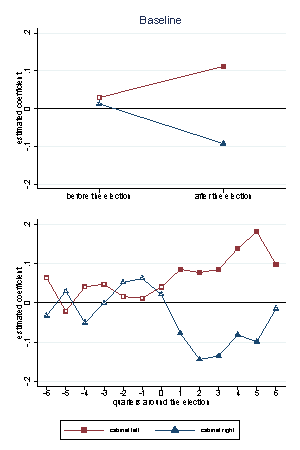
\includegraphics[width=\linewidth]{../results/applications/app_graphs_baseline.pdf}
		{\scriptsize Note: These figures show the time evolution of refugee inflows as estimated in fixed effects regression with a set of dummies for before and after the election or a set of dummies for different quarters before and after an election in a quarter t = 0. Significant coefficients are indicated by filled plot markers. Periods in which the two coefficients are significantly different from each other are indicated with a grey background.\par}
	\end{minipage}
\end{figure}

In line with the literature and the results of \citet{hatton2016}, we find that measures of political oppression and violence in the host country are positively correlated with the number of asylum applications. The negative significant coefficient of the log origin country real GDP per capita suggests that also adverse economic conditions in the host countries drive asylum applications. As bad economic conditions are, however, often a byproduct of wars and political instability, this does not mean that asylum seekers leave their home country primarily for economic reasons. Moreover, we find a small negative effect of the unemployment rate in the destination country, which could indicate both, that a higher unemployment rate reduces the attractiveness of a destination country or that in times of higher unemployment more restrictive asylum policies are implemented. Interestingly, in contrast to \citet{hatton2016}, our results (which are based on a different sample of countries) indicate that a higher GDP per capita in the destination country is associated with fewer asylum applications. 

To gain a more precise understanding, we test the model with individual dummies for different quarters before and after an election. The results of the main coefficients of interest are presented in Table \ref{app_graph2_coef} and illustrated graphically in Figure \ref{main_results_app}. The detailed analysis confirms that the turning point is really the quarter following the election. Before the election the cabinet coefficients are not different from average policies. Moreover, the difference between the coefficients for left-wing and right-wing cabinets is never statistically significant. However, after the election almost all cabinet coefficients become significant and substantially larger. Again, there is a remarkable difference in the sign of the coefficients related to the different types of parties. The signs of the left-wing parties are all positive, whereas those of the right-wing parties are consistently negative. As a consequence, the difference between the left-wing and right-wing cabinet coefficients is always significant after the election. Again, the result suggests that both left-wing and right-wing cabinets choose moderate policies before the election and less moderate policies after the election. 
%MARTINA: - delete that sentence as it doesn't fit anymore when we change the order of the paragraphs 
%As highlighted in the section \ref{sec:robustness}, the result is robust to the specifications discussed with respect to the two-period model above. 

\begin{table}[htbp]\centering
\def\sym#1{\ifmmode^{#1}\else\(^{#1}\)\fi}
\caption{Coefficients Graph 2}
\begin{tabular}{l*{2}{c}}
\hline\hline
                    &\multicolumn{1}{c}{(1)}&\multicolumn{1}{c}{(2)}\\
                    &\multicolumn{1}{c}{left}&\multicolumn{1}{c}{right}\\
\hline
 6 quarters before the election&      0.0555\sym{*}  &     -0.0244         \\
                    &    (0.0275)         &    (0.0365)         \\
[1em]
 5 quarters before the election&     -0.0294         &      0.0385         \\
                    &    (0.0295)         &    (0.0311)         \\
[1em]
 4 quarters before the election&      0.0333         &     -0.0422         \\
                    &    (0.0366)         &    (0.0385)         \\
[1em]
 3 quarters before the election&      0.0398         &     0.00650         \\
                    &    (0.0439)         &    (0.0302)         \\
[1em]
 2 quarters before the election&     0.00828         &      0.0600         \\
                    &    (0.0358)         &    (0.0385)         \\
[1em]
 1 quarters before the election&     0.00414         &      0.0701         \\
                    &    (0.0425)         &    (0.0363)         \\
[1em]
Quarter of the election&      0.0325         &      0.0293         \\
                    &    (0.0393)         &    (0.0374)         \\
[1em]
 1 quarters after the election&      0.0775\sym{*}  &     -0.0698         \\
                    &    (0.0373)         &    (0.0364)         \\
[1em]
 2 quarters after the election&      0.0697\sym{*}  &      -0.136\sym{***}\\
                    &    (0.0346)         &    (0.0338)         \\
[1em]
 3 quarters after the election&      0.0774\sym{*}  &      -0.127\sym{**} \\
                    &    (0.0339)         &    (0.0448)         \\
[1em]
 4 quarters after the election&       0.131\sym{***}&     -0.0733         \\
                    &    (0.0315)         &    (0.0384)         \\
[1em]
 5 quarters after the election&       0.173\sym{***}&     -0.0904\sym{**} \\
                    &    (0.0288)         &    (0.0350)         \\
[1em]
 6 quarters after the election&      0.0899\sym{***}&    -0.00688         \\
                    &    (0.0264)         &    (0.0296)         \\
\hline
Observations        &       23705         &       23705         \\
\hline\hline
\multicolumn{3}{l}{\footnotesize Standard errors in parentheses}\\
\multicolumn{3}{l}{\footnotesize \sym{*} \(p<0.05\), \sym{**} \(p<0.01\), \sym{***} \(p<0.001\)}\\
\end{tabular}
\end{table}




% MARTINA: If we have an extra section Robustness I think it makes sense to put this entire paragraph in the robustness section. Or leave it here and restructure such that we have first applications then robustness applications and then decisions and robustness for decisions - I think the second option makes more sense - discuss the robustness checks directly after the application results and just add that in the online appendix we do also various other robustness checks and all stays the same, maybe just with bulletpoints as in the current robustness section, but we have to update it as some robustness checks have changed
% MARTINA: right now the robustness section is anyway only about applications and talks about several things that we no longer do or no longer show in the online appendix , so after the decision results we should add some sentences on robustness checks here as well and refer to the online appendix for detailed results

As evident from Table \ref{app_table_base-R6} and Figure \ref{graph_robustness}, our results are robust to different specifications.
% MARTINA made some adjustments to be in line with the most recent results table. It seems like you had some other table when describing the results - this is the order of the table basline to R6.
 Column (R1) and (R2)  offer variants with different fixed effects and yield an almost identical outcome.\footnote{In column (R1) we include origin and destination fixed effects separately along with quarter-year dummies and in column (R2) we estimate a variant with origin-time fixed effects along with destination fixed effects. In both specifications we moreover include two time-constant country-pair specific variables, the (log) distance between the capital cities and the stock of migrants of origin country $i$ in destination country $j$ in 2000.} In column (R3), we test a dynamic variant of the model by considering how past asylum policies affect our results. In particular, we add the (log) five year average of past asylum applications per capita. The coefficients are highly significant and positive, suggesting that asylum policies are path-dependent, but our main results remain unaffected. Column (R5) introduces the position of the cabinet separately to test for level differences in the behavior of parties. The results suggest that there are no significant level differences and our main results remain stable as well. Finally, column (R6) adds Hatton's asylum policy index to account formal changes in asylum policies and to disentangle these de jure changes from de facto changes in the administration and implementation of asylum policies by the ruling government. The results indicate that the asylum policy index is highly relevant confirming \citet{hatton2016}. Interestingly, the estimates of our coefficients of interest remain very stable indicating that both measures are crucial determinants of asylum policy outcomes, but capture different elements of actual asylum policies. When splitting up Hatton's asylum policy index in its three sub-components (column (R7)), the drivers behind its impact seem to be policies on processing and welfare, whereas the access policies are only significant at the 10\% level.
 % !!! MARTINA: the coefficient of the access policies has 2 stars, which means 1% level, three stars mean 0.1% level, so also the access policy index is pretty significant. But we could argue that it has the smalles coefficient in our specification whereas it has the largest coefficient in hatton's paper.
   A potential explanation might be that the policies captured by our political-economy set-up mainly refer to the access of asylum seekers to the destination countries. Access policies, such as border controls, can be changed rather quickly and are under the direct administration of the government. 
   
% MARTINA: I would suggest to put that paragraph further up, because now we have the two models in one graph

%To gain a more precise understanding, we test the model with individual dummies for different quarters before and after an election. The results of the main coefficients of interest are presented in Table \ref{app_graph2_coef} and illustrated graphically in Figure \ref{main_results_app}. The detailed analysis confirms that the turning point is really the quarter following the election. Before the election the cabinet coefficients are not different from average policies. Moreover, the difference between the coefficients for left-wing and right-wing cabinets is never statistically significant. However, after the election almost all cabinet coefficients become significant and substantially larger. Again, there is a remarkable difference in the sign of the coefficients related to the different types of parties. The signs of the left-wing parties are all positive, whereas those of the right-wing parties are consistently negative. As a consequence, the difference between the left-wing and right-wing cabinet coefficients is always significant after the election. Again, the result suggests that both left-wing and right-wing cabinets choose moderate policies before the election and less moderate policies after the election. As highlighted in the section \ref{sec:robustness}, the result robust to the specifications discussed with respect to the two-period model above. 


 

\begin{figure}
	\caption{First-time asylum applications per capita: predicted pattern - R1 to R6}
	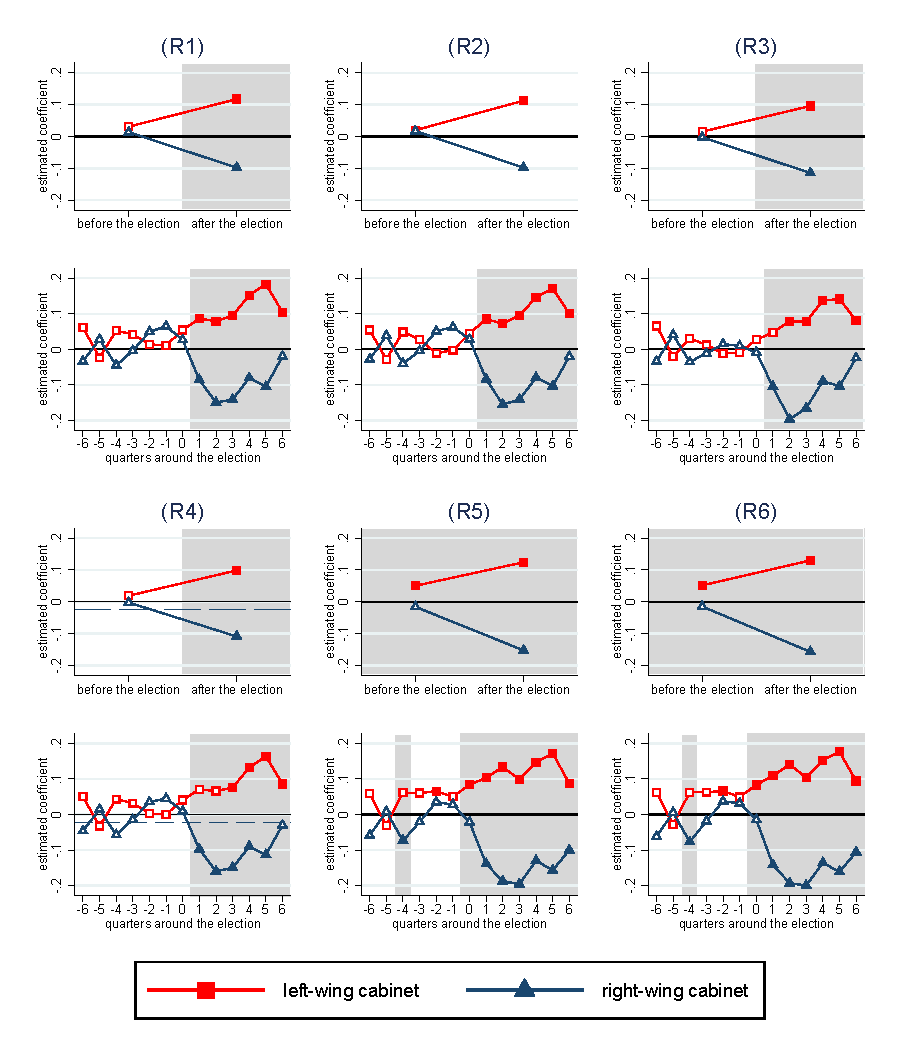
\includegraphics[width=1\textwidth]{../results/applications/app_graphs_R1-R6.pdf}
	\scriptsize{Note: These figures show the time evolution of refugee inflows as estimated in fixed effects regression with a set of dummies for before and after the election or a set of dummies for different quarters before and after an election in a quarter t = 0. Significant coefficients are indicated by filled plot markers. Periods in which the two coefficients are significantly different from each other are indicated with a grey background. The navy dashed line in sub-figure R4 shows the average inflow of asylum seekers under right-wing cabinets in periods outside the election period. Significance of the coefficients of the right-wing cabinet in sub-figure R4 is reported for the distance to this average non-election period effect.}
	\label{graph_robustness}
\end{figure} 

\subsection{Decisions}

The determinants of asylum decisions based on the fixed effects regression specified in equation (1) with quarter-year dummies and destination-origin fixed effects (not reported) are presented in Table \ref{dec_table1_baseline}. In column (1) we use the acceptance rate, i.e. the number of positive decisions as a share of all decisions, as dependent variable.\footnote{We define all decisions as all positive decision plus the negative decisions} In column (2) and column (3) we then also assess the recognition rates for the two different statuses,  refugee status and temporary protection, separately. With respect to the acceptance rate we do not find any significant deviation from average policies before the election, but after the election the coefficients for right-wing and left-wing cabinets clearly differ. Again, the sign of the after-election coefficients depends on the identity of the cabinet. Left-wing cabinets are associated with a lower recognition rate and right-wing cabinets with a higher one. As evident from the analysis of the refugee status rate (Column (2)) and the temporary protection rate (Column (3)), the effect is driven by a decline in the refugee status rate under left-wing cabinets and a strong increase in the temporary protection rate under right-wing cabinets after the election. 
[Add level differences]
% MARTINA: In case you want the graph of all three with the cabinet right dummy here or if I should include the cabinet right in the table again let me know... if not I would suggest to just discuss it later together with other robustness checks and refer to the online appendix for the graphs and tables ...
 When examining asylum decisions at a quarterly level, a similar picture emerges which is illustrated in Figure \ref{dec_graphs_baseline}.  Before the election, policies remain rather similar, but differ clearly after the election. Again, the refugee status rate is lower under left-wing cabinets and the use of temporary protection more widespread under right-wing governments. In total, the pattern that was observed in the case of asylum applications seems to be reversed.

The finding of a reversed electoral cycle and lower recognition rate under left-wing cabinets appears counter-intuitive. One potential explanation for our finding is that changes in the number of asylum applications mechanically translate into changes in the decision outcome. While a government can quickly adjust access policies, e.g. via stricter enforcement of border controls, the decisions on asylum applications are more difficult to influence. These decisions are based on existing laws for which changes take time and require the consent of the parliament. Moreover, independent judiciaries pose restrictions for changes in the decision-making process. In total, the decision process is likely to be stable over time. In that case  recognition rates strongly depend on the characteristics of the applicants. If more restrictive access policies under right-wing cabinets lead to the selection of refugees that on average are more entitled to asylum than a less selected group entering under a left-wing cabinet, the asylum recognition rate under right-wing cabinets must be higher than under left-wing cabinets. Analogously, an increase / a decrease of asylum applications under left-wing / right-wing cabinets after the election should translate into a decline / an increase of the recognition rate.


\begin{figure}
	\caption{Asylum decisions per capita: predicted pattern - baseline}
	\centering
	\begin{minipage}{1\textwidth} 
		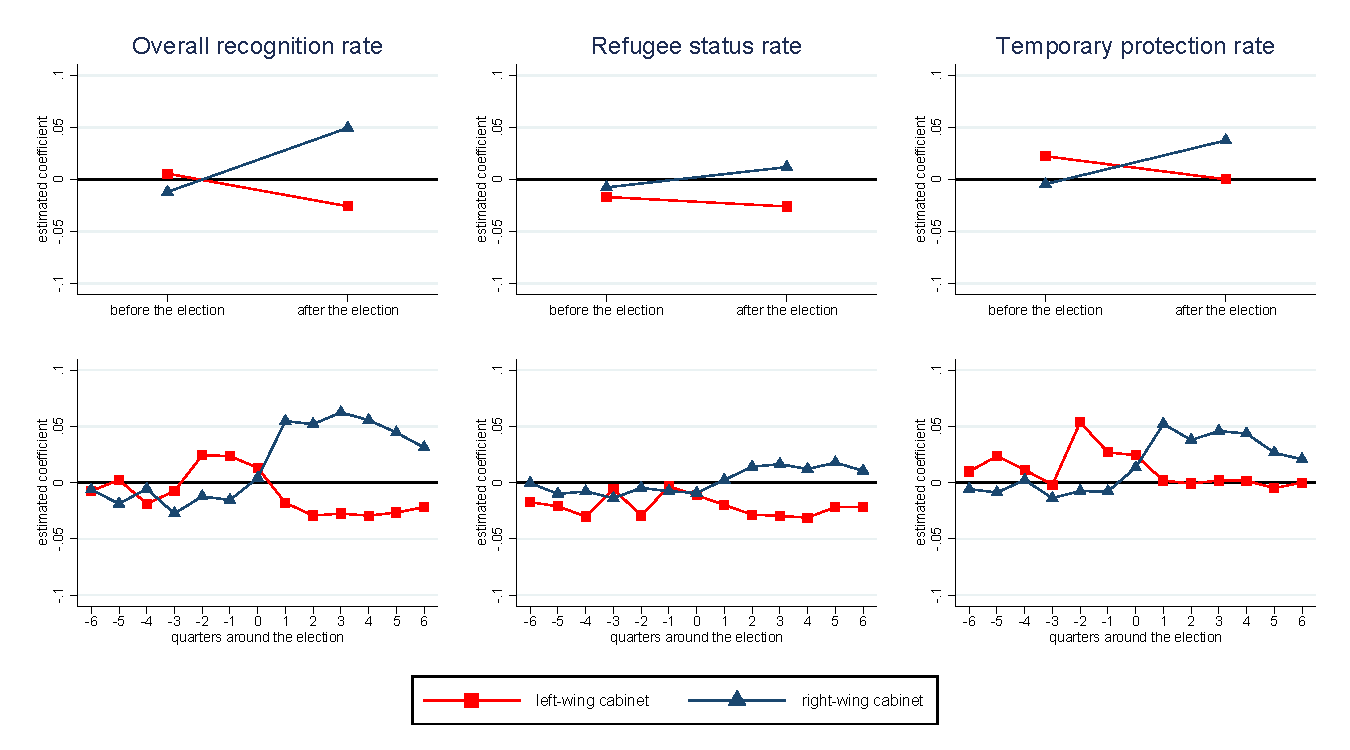
\includegraphics[width=\linewidth]{../results/decisions/dec_graphs_baseline.pdf}
		{\scriptsize Note: These figures show the time evolution of the acceptance rate, the refugee status rate and the temporary protection rate as estimated in fixed effects regression with a set of dummies for before and after the election or a set of dummies for different quarters before and after an election in a quarter t = 0. Significant coefficients are indicated by filled plot markers. Periods in which the two coefficients are significantly different from each other are indicated with a grey background. \par}
	\end{minipage}
\label{dec_graphs_baseline}
\end{figure}

\begin{table}[!ht]\centering \scriptsize
\def\sym#1{\ifmmode^{#1}\else\(^{#1}\)\fi}
\caption{Determinants of asylum decisions}
\begin{tabular}{l*{3}{c}}
\hline\hline
Dependent variable                    &\multicolumn{1}{c}{Acceptance rate}&\multicolumn{1}{c}{Refugee status rate}&\multicolumn{1}{c}{Temporary protection rate}\\
\hline
Political Terror Scale&      0.0269\sym{*}  &      0.0297\sym{**} &    -0.00281         \\
                    &    (0.0109)         &   (0.00860)         &   (0.00629)         \\
[0.5em]
Civic Liberty (FHI) &      0.0345         &      0.0219         &      0.0126         \\
                    &    (0.0226)         &    (0.0145)         &   (0.00993)         \\
[0.5em]
Political Rights (FHI)&    -0.00792         &    -0.00961         &     0.00169         \\
                    &    (0.0199)         &    (0.0116)         &   (0.00924)         \\
[0.5em]
Quarterly civil war &      0.0532\sym{***}&      0.0160\sym{***}&      0.0372\sym{***}\\
battle death (000s)                    &   (0.00503)         &   (0.00323)         &   (0.00263)         \\
[0.5em]
Log origin country &     -0.0227         &     -0.0135         &    -0.00921         \\
real GDP per capita                    &    (0.0322)         &    (0.0252)         &    (0.0111)         \\
[0.5em]
Log destination country&       0.223\sym{*}  &      -0.131\sym{*}  &       0.354\sym{***}\\
 quarterly real GDP per capita                    &    (0.0863)         &    (0.0598)         &    (0.0777)         \\
[0.5em]
Quarterly unemployment &  -0.0000658         &    -0.00402\sym{*}  &     0.00395\sym{*}  \\
rate at destination                    &   (0.00115)         &   (0.00161)         &   (0.00161)         \\
[0.5em]
Cabinet position left * &     0.00568         &     -0.0168\sym{**} &      0.0225\sym{***}\\
 Before the election                   &   (0.00771)         &   (0.00530)         &   (0.00483)         \\
[0.5em]
Cabinet position left * &     -0.0256\sym{**} &     -0.0257\sym{***}&   0.0000830         \\
 After the election                   &   (0.00760)         &   (0.00534)         &   (0.00377)         \\
[0.5em]
Cabinet position right * &     -0.0118         &    -0.00716         &    -0.00469         \\
 Before the election                   &   (0.00738)         &   (0.00564)         &   (0.00519)         \\
[0.5em]
Cabinet position right * &      0.0496\sym{***}&      0.0123\sym{**} &      0.0373\sym{***}\\
After the election                    &   (0.00904)         &   (0.00416)         &   (0.00823)         \\
\hline
Observations        &       12921         &       12921         &       12921         \\
Adjusted \(R^{2}\)  &       0.134         &       0.083         &       0.067         \\
Mean dependent variable&       0.159         &      0.0866         &      0.0725         \\
Fixed Effects       &       D x O         &       D x O         &       D x O         \\
Destination dummies &          No         &          No         &          No         \\
Quarter-Year dummies&         Yes         &         Yes         &         Yes         \\
\hline\hline
\multicolumn{4}{l}{Standard errors in parentheses \sym{*} \(p<0.05\), \sym{**} \(p<0.01\), \sym{***} \(p<0.001\)}\\
\end{tabular}
\label{dec_table1_baseline}
\end{table}




\section{Robustness Checks}\label{sec:robustness}

% MARTINA: I would drop the entire section and incorporate it into the results section - and if we keep it we have to rewrite it, because in our robustness checks we do no longer do all the things and moreover there are no rubustness checks for the decision analysis dicussed.
 
%In order to account for the fact that in general refugee inflows might be different under right and left cabinets we include a dummy for the incumbent's cabinet position in addition to the interaction terms.  As the coefficient is very small and insignificant and the main results do not change, we decide to drop the dummy for the incumbent's cabinet position in the main specification.  

Our robustness checks (available upon request) show that our main results are very stable across a large number of different specifications of our regression equation (1). Among others, we control for the average asylum applications per capita in the previous 5 years, which indicates that election outcomes are not influenced by previous refugee inflows.  A further concern is that some of our effects might be driven by the change in the data collection method by Eurostat in 2008. In order to account for that, we therefore also conduct a robustness check including a dummy which is equal to 1 if the year is 2008 or later and equal to zero if the year is 2002 to 2007. As the coefficient of this dummy is small and insignificant and the results do not change, we are confident that change in the collection method does not influence our results. Several other robustness checks, moreover,  show that our results are not sensible to
\begin{itemize}
\itemsep0em 
\item  using the log of the number of first-time asylum applications per capita in the in the \textbf{origin} country as our dependent variable 
\item using  the current values of the origin country control variables instead of averages of the current and the past three quarters 
\item clustering the standard errors on the destination-origin level
\item normalizing the cabinet position on the country level before computing the cabinet position dummies (left and right)
\item leaving missing data on quarterly  first-time asylum applications for 2008 and 2009 missing instead of imputing it from the total applications
\item choosing  different cutoffs  for dropping countries pairs with few applications (one and three average applications per quarter)
\item looking only at five or four quarters around the election 
\end{itemize}
%Regression tables and graphs for all robustness checks are presented in the online appendix. 
Finally, we test whether our results depend on the sample of countries used. The results only change marginally  when we include Cyprus in the sample of destination countries. Moreover, when adding very small countries in terms of first-time applications (Estonia, Latvia, Lithuania, Portugal, Malta and Slovenia), the main pattern is still visible in the data.\footnote{Note that for each sample of destination countries we adjust the sample of origin countries such that in total the origin countries account for more than 90 percent of all first-time applications in the destination countries between 2002 and 2014.}  


\section{Conclusion}\label{sec:conclusion}

We examine the impact of elections and parties on first-time asylum applications based on a large bilateral panel data set comprising 12 European destination countries and their 51 most relevant origin countries during the time period 2002 to 2014. Our findings suggest that  the number of asylum applicants under left- and right-wing parties converges before elections and differs thereafter. In conclusion, our results clearly show a strong impact of elections and parties on first-time asylum applications. This highlights the need to better model the influence of political economy factors such as elections or interactions among receiving countries when analyzing the determinants of refugees inflows \citep{gorlach2017}. 

Our analysis shows that asylum policies in the EU are partly driven by national elections. First, our findings imply that staggered election schedules further deteriorate the already highly heterogeneous EU asylum policy. This in turn is likely to generate harmful migration deviation effects within the EU. \citet{thielemann2006} points out that with heterogeneous asylum policies each state's actions generate externalities for other states that potentially cause controversies between states. Second, our findings imply that the chance of refugees for being recognized depends on factors that should not play a role according to the normative fundamentals of asylum policies, such as the Geneva Convention. \citet{neumayer2005} shows that recognition rates for asylum seekers from the same countries of origin varies considerably across Western European countries over the period from 1980 to 1999. He argues that this variation constitutes unfair and discriminatory treatment of asylum claims. Along the same line, our findings generate a further argument in favor of a harmonized common EU asylum policy which should be less influenced by national electoral cycles. 



Further research is needed to uncover the precise mechanisms underlying our results. Our analysis cannot disentangle which part of the effects on refugee inflows are driven by the demand side, i.e. the refugees selecting into different countries depending on current asylum policies, or the supply side, i.e. the incumbent government adjusting asylum policies.  Survey data on the pre-existing knowledge of asylum seekers and their decision strategies might allow to analyse these questions in the future. 
 


%--------------------------------------------------------------------------------------------------
\pagebreak
\bibliographystyle{apalike}
\bibliography{refugee_election}
%\appendix
%%--------------------------------------------------------------------------------------------------
%\section{Additional Figures}\label{app_fig}
%\input{app_figures}
%%--------------------------------------------------------------------------------------------------

\end{document}

